\chapter{Dimension}

In this chapter, all rings are assumed to be commutative, and algebras are associative, commutative, and unital.

Let A be a ring. If a is an ideal of A and n is a negative integer, we set \(a^{n} = A\) . For every prime ideal p of A, we denote by \(\kappa(\mathfrak{p})\) the residue field of the local ring \(A_{p}\) ; it is canonically isomorphic to the field of fractions of the ring A/p (II, § 3, no. 1, prop. 2). If A is local, we denote by \(m_{A}\) its maximal ideal, and \(\kappa_{A} = A/m_{A} = \kappa(m_{A})\) its residue field.

Let \(\rho: A \to B\) be a ring homomorphism. We denote by \(^a\rho\) the continuous map from \(\operatorname{Spec}(B)\) to \(\operatorname{Spec}(A)\) associated with \(\rho\) (II, § 4, no. 3). We say (V, § 2, no. 1, def. 1) that a prime ideal q of B lies over the prime ideal p of A if p is the image of q under \(^a\rho\) , that is, if \(\rho^{-1}(q) = p\) . Let M be a B-module; when we consider M as an A-module, it is always the A-module structure \(\rho_*(M)\) defined by the external law \((a, m) \mapsto \rho(a).m\) (A, II, p. 30).

Let M be an A-module. If U (resp. V) is an additive subgroup of A (resp. M), we denote by UV or U.V the additive subgroup of M generated by the products uv, for \(u \in U\) and \(v \in V\) . If S is a subset of A, we denote by SM the submodule \(\sum_{s \in S} sM\) of M; the ideal of A generated by S is equal to SA and we have S.M = SM.

\section{KRULL DIMENSION OF A RING}

\subsection{Krull dimension of a topological space}

DEFINITION 1. --- Let I be an ordered set. A nonempty finite subset of I that is totally ordered is called a chain of I. Let c be a chain of I; the least and greatest elements of c are called the endpoints of c. The integer Card(c) - 1 is called the length of c. The inclusion relation on the set of subsets of I induces an order relation on the set of chains of I. A chain c of I is said to be saturated if it is maximal among the chains of I having the same endpoints as c.

To denote a chain c of length n, we shall often write: "the chain", \(i_{0} < \cdots < i_{n}\) , where the \(i_{k}\) are the elements of c indexed in strictly increasing order by the integers from 0 to n.

Let X be a topological space. We equip the set of irreducible closed subsets of X (II, § 4, no. 1, def. 1) with the order relation defined by inclusion. When we speak of a chain of irreducible closed subsets of X, it is always a chain in the sense of this order relation.

DEFINITION 2. --- We call the Krull dimension of the topological space X, and denote by dim kr(X) or simply dim(X), the supremum in \(\overline{\mathbf{R}}\) of the set of lengths of chains of irreducible closed subsets of X.

For every point x in X, we call the Krull dimension of X at x and denote it by \(\dim_{x}(X)\); it is the infimum of the dimensions of open neighborhoods of x.

We have \(\dim(\emptyset) = -\infty\) . On the other hand, if X is nonempty, the closure of any point of X is a closed irreducible subset of X (II, § 4, no. 1, prop. 2), and hence the dimension of X is either +∞ or a positive integer. Suppose that X is separated and nonempty; then every irreducible subset of X is reduced to a point, and X has dimension 0.

\pandocbounded{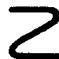
\includegraphics[keepaspectratio]{images/part001_0d60a61e.jpg}}

The definition of Krull dimension is therefore devoid of interest for separated spaces, but it is especially well suited to the topological spaces encountered in Commutative Algebra (spectra of rings, *schemes*, \ldots). In this chapter, no confusion is to be feared with other notions of dimension for topological spaces (for example, that of Lebesgue), and we will simply say “dimension” for “Krull dimension.”

PROPOSITION 1. --- Let X be a topological space.

\begin{enumerate}
\def\labelenumi{\alph{enumi})}
\item
  If Y is a subspace of X, we have \(\dim(\mathbf{Y}) \leqslant \dim(\mathbf{X})\) , and \(\dim_y(\mathbf{Y}) \leqslant \dim_y(\mathbf{X})\) for every point \(y\) of Y.
\item
  Let \(x\) be a point of \(X\) and \(V\) a neighborhood of \(x\) in \(X\) . We have \(\dim_x(X) = \dim_x(V)\) .
\item
  Let \((\mathbf{X}_i)_{i\in I}\) be a finite family of closed subsets of X such that \(\mathbf{X} = \bigcup_{i\in I}\mathbf{X}_i\) . We have
\end{enumerate}

\(\dim(X) = \sup_{i \in I} \dim(X_i)\)and, for every point \(x\) of \(X\)\(\dim_x(X) = \sup_{i \in J_x} \dim_x(X_i)\)\(J\)\(i \in J\)\(x \in X\) , one has

where  denotes the set of  such that .\[
\mathrm{J} _ {x}
\]

Let us prove a). If Z is an irreducible closed subset of Y, its closure \(\overline{Z}\) in X is irreducible (II, § 4, no. 1, prop. 2) and one has \(\overline{Z} \cap Y = Z\) . Thus, every chain \(c\) of closed irreducible subsets of Y defines, by passing to the closure in X, a chain of closed irreducible subsets of X, of the same length as \(c\) . The inequality \(\dim(Y) \leqslant \dim(X)\) follows from this. If U is an open subset of X containing a point \(y\) of Y, we therefore have \(\dim(U \cap Y) \leqslant \dim(U)\) , whence \(\dim_y(Y) \leqslant \dim_y(X)\) .

We prove \(b\) . By definition \(\dim_{x}(X) \leqslant \dim_{x}(V)\) , and the opposite inequality follows from \(a\) ).

We prove \(c\) ). Let \(Z_{0} \subset \ldots \subset Z_{n}\) be a chain of irreducible closed subsets of X. We have \(Z_{n} = \bigcup_{i \in I} (Z_{n} \cap X_{i})\) and each of the sets \(Z_{n} \cap X_{i}\) is closed in \(Z_{n}\) ;

since I is finite, \(Z_{n}\) is contained in one of the \(X_{i}\) . Consequently, we have \(\dim(X) \leqslant \sup_{i} \dim(X_{i})\) , whence equality by \(a\) ).

Now let \(x\) be a point of \(X\) and \(n = \sup_{i \in J_x} \dim_x(X_i)\) , where \(J_x\) is as in the statement. We have \(\dim_x(X) \geqslant n\) by \(a\) ), and, to establish the equality, we may assume \(n\) finite. For every \(i \in J_x\) , let \(U_i\) be an open neighborhood of \(x\) in \(X\) such that \(\dim(U_i \cap X_i) \leqslant n\) . Put \(U = (\bigcap_{i \in J_x} U_i) \cap (\bigcap_{i \in I - J_x} \complement X_i)\) ; the set \(U\) is open in \(X\) . Moreover, we have \(\dim(U) = \sup_{i \in J_x} \dim(U \cap X_i) \leqslant n\) by the preceding paragraph, hence \(\dim_x(X) \leqslant n\) .

COROLLARY. --- a) The dimension of the topological space X is the supremum of the dimensions of its irreducible components (II, § 4, no. 1, definition 2).

\begin{enumerate}
\def\labelenumi{\alph{enumi})}
\setcounter{enumi}{1}
\tightlist
\item
  Let \(x\) be a point of \(X\) . We have \(\dim_x(X) \geqslant \sup_i \dim_x(X_i)\) , where \(X_i\) runs through the family
\end{enumerate}
of irreducible components of X that contain x; there is equality if x has a neighborhood V which has only finitely many irreducible components (which is the case for example if V is Noetherian).


The first assertion is immediate since the chains of irreducible closed subsets of X are the chains of irreducible closed subsets of the irreducible components of X (II, § 4, no. 1, prop. 5). The inequality \(\dim_x(X) \geqslant \sup_i \dim_x(X_i)\) follows

from prop. 1, a). Let V be a neighborhood of x which has only finitely many irreducible components, and let \((\mathrm{V}_{j})_{j\in\mathbb{J}}\) be the family of irreducible components of V that contain x. It follows from prop. 1, b) and c) that we have

\[
\dim_ {x} (X) = \dim_ {x} (V) = \sup _ {j \in J} \dim_ {x} (V _ {j});
\]

we conclude by noting that each of the \(V_{j}\) is contained in one of the \(X_{i}, i \in J_{x}\) , and that consequently we have \(\sup_{j \in J} \dim_{x}(V_{j}) \leqslant \sup_{i \in J_{x}} \dim_{x}(X_{i})\) .

PROPOSITION 2. — Let X be a topological space. We have \(\dim(X) = \sup_{x \in X} \dim_x(X)\) .

Indeed, by definition we have \(\dim(X) \geqslant \dim_x(X)\) for every \(x \in X\) . On the other hand, if \(Z_0 \subset \ldots \subset Z_n\) is a chain of irreducible closed subsets of \(X\) , for all \(x \in Z_0\) and every open neighborhood \(U\) of \(x\) , the sets \(Z_0 \cap U, \ldots, Z_n \cap U\) form a chain of irreducible closed subsets of \(U\) (II, § 4, no. 1, prop. 7). We therefore have \(\dim_x(X) \geqslant n\) , whence \(\dim(X) \leqslant \sup_{x \in X} \dim_x(X)\) .

COROLLARY. — If \((\mathrm{X}_{\alpha})_{\alpha\in\mathbf{A}}\) is an open covering, or a locally finite closed covering, of a topological space X, we have

\[
\dim (X) = \sup _ {\alpha \in A} \dim (X _ {\alpha}).
\]

It suffices to show that, for every point \(x\) of \(X\), one has \(\dim_x(X) = \sup_{\alpha \in A_x} \dim_x(X_\alpha)\), where \(A_x\) is the set of \(\alpha \in A\) such that \(x \in X_\alpha\). This is clear in the case of an open covering, and follows from Proposition 1, c), in the case of a locally finite closed covering.

\subsection{Codimension of a closed subset}

DEFINITION 3. --- Let X be a topological space.

\begin{enumerate}
\def\labelenumi{\alph{enumi})}
\item
  If Y is a closed irreducible subset of X, one calls the codimension of Y in X the supremum in \(\overline{\mathbf{R}}\) of the lengths of the chains of irreducible closed subsets of X for which Y is the smallest element.
\item
  If Y is a closed subset of X, we call the codimension of Y in X, and denote it by \(\text{codim}(Y, X)\) the infimum in \(\overline{\mathbf{R}}\) of the codimensions, in X, of the irreducible components of Y.
\end{enumerate}

Remarks. --- 1) The codimension of a closed subset Y of X is therefore the infimum of the codimensions of the irreducible closed subsets of Y. We have \(\mathrm{codim}(\emptyset, \mathrm{X}) = +\infty\) and, if X is nonempty, \(\mathrm{codim}(\mathrm{X}, \mathrm{X}) = 0\) . Every nonempty closed subset of X contains an irreducible closed subset (II, § 4, no. 1, prop. 5); hence the codimension in X of a closed subset Y is always a nonnegative integer, or \(+\infty\) . It is zero if and only if Y contains an irreducible component of X.

\begin{enumerate}
\def\labelenumi{\arabic{enumi})}
\setcounter{enumi}{1}
\tightlist
\item
  If Y is a nonempty closed subset of X, then codim(Y, X) ≤ dim(X). Moreover, dim(X) = sup codim(Y, X), where Y ranges over the set of irreducible closed subsets.
\end{enumerate}

If Y and Y' are two closed subsets of X such that Y' ⊂ Y, then codim(Y, X) ≤ codim(Y', X).

\begin{enumerate}
\def\labelenumi{\arabic{enumi})}
\setcounter{enumi}{2}
\tightlist
\item
  Let Y be a closed subset of the topological space X and \((\mathrm{X}_{\alpha})_{\alpha\in\mathrm{A}}\) (resp. \((\mathrm{Y}_{\beta})_{\beta\in\mathrm{B}}\) ) the family of irreducible components of X (resp. of Y). For every \(\beta\in B\) , denote by \(\mathrm{A}(\beta)\) the set of \(\alpha\in A\) such that \(Y_{\beta}\subset X_{\alpha}\) . Since every irreducible subset of X is contained in one of the \(X_{\alpha}\) (II, § 4, no. 1, prop. 5), it follows from Def. 3 that we have:
\end{enumerate}

\[
\operatorname{codim} (Y, X) = \inf _ {\beta \in B} \sup _ {\alpha \in A (\beta)} \operatorname{codim} (Y _ {\beta}, X _ {\alpha}).
\]

\begin{enumerate}
\def\labelenumi{\arabic{enumi})}
\setcounter{enumi}{3}
\tightlist
\item
  Let \((\mathbf{Y}_i)_{i\in I}\) be a finite family of closed subsets of X and \(\mathbf{Y} = \bigcup_{i\in I}\mathbf{Y}_i\) ; one has
\end{enumerate}

\[
\operatorname{codim} (\mathrm{Y}, \mathrm{X}) = \inf _ {i \in \mathrm{I}} \operatorname{codim} (\mathrm{Y} _ {i}, \mathrm{X}).
\]

Indeed, every irreducible component of Y is contained in one of the \(Y_{i}\) .

PROPOSITION 3. --- Let X be a topological space.

\begin{enumerate}
\def\labelenumi{\alph{enumi})}
\tightlist
\item
  For every nonempty closed subset Y of X, we have
\end{enumerate}

\[
\dim (\mathrm{Y}) + \operatorname{codim} (\mathrm{Y}, \mathrm{X}) \leqslant \dim (\mathrm{X}).
\]

\begin{enumerate}
\def\labelenumi{\alph{enumi})}
\setcounter{enumi}{1}
\tightlist
\item
  If Y, Z, and T are closed subsets of X such that Y ⊂ Z ⊂ T, then
\end{enumerate}

\[
\operatorname{codim} (\mathrm{Y}, \mathrm{Z}) + \operatorname{codim} (\mathrm{Z}, \mathrm{T}) \leqslant \operatorname{codim} (\mathrm{Y}, \mathrm{T}).
\]

It suffices to prove the assertion \(a)\) in the case where \(\dim(X)\) is finite. In this case, \(\dim(Y)\) and \(\operatorname{codim}(Y, X)\) are finite. There exists a chain \(Y_0 \subset \ldots \subset Y_n\) of closed irreducible subsets of \(Y\), of length \(n = \dim(Y)\) and a chain \(Y_n \subset \ldots \subset Y_{n+p}\) of closed irreducible subsets of \(X\), of length \(p \geqslant \operatorname{codim}(Y, X)\). It follows that \(\dim(X) \geqslant n + p\), whence . To establish \(a)\)\(b)\), one may assume \(Y\) irreducible. Since we have \(\operatorname{codim}(Y, Z) \leqslant \operatorname{codim}(Y, T)\), the inequality is proved if \(\operatorname{codim}(Y, Z) = +\infty\). Otherwise, let \(Z_0\) be an irreducible component of \(Z\) containing \(Y\) and such that \(\operatorname{codim}(Y, Z) = \operatorname{codim}(Y, Z_0)\). We have \(\operatorname{codim}(Z, T) \leqslant \operatorname{codim}(Z_0, T)\), and one sees, as above, that \(\operatorname{codim}(Y, Z_0) + \operatorname{codim}(Z_0, T) \leqslant \operatorname{codim}(Y, T)\), whence \(b)\).

DEFINITION 4. --- A topological space X is said to be catenary if, for every pair (Y, Z) of irreducible closed subsets of X such that Y ⊂ Z, every saturated chain of irreducible closed subsets with endpoints Y and Z has length codim(Y, Z).

It is equivalent to say that, for every pair (Y, Z) of irreducible closed subsets of X such that codim(Y, Z) is finite, all saturated chains with endpoints Y and Z have the same length, and that, for every pair (Y, Z) such that codim(Y, Z) = +∞, there exists no saturated chain with endpoints Y and Z.

Every closed subspace of a catenary space is catenary. For a space to be catenary, it is necessary and sufficient that its irreducible components be catenary.

PROPOSITION 4. --- Let X be a topological space. For X to be catenary, it is necessary and sufficient that, for every triple (Y, Z, T) of irreducible closed subsets of X such that Y ⊂ Z ⊂ T, one has:

\[
\operatorname{codim} (\mathrm{Y}, \mathrm{T}) = \operatorname{codim} (\mathrm{Y}, \mathrm{Z}) + \operatorname{codim} (\mathrm{Z}, \mathrm{T}).
\]

Suppose X is catenary. In view of prop. 3, b), it suffices to prove the relation when codim(Y, Z) and codim(Z, T) are finite. By concatenating a saturated chain of irreducible closed subsets with endpoints Y and Z, of length codim(Y, Z), and a saturated chain of irreducible closed subsets with endpoints Z and T, of length codim(Z, T), one obtains a saturated chain with endpoints Y and T, of length codim(Y, Z) + codim(Z, T). But, since X is catenary, this length is necessarily equal to codim(Y, T).

Conversely, suppose we have \(\operatorname{codim}(\mathbf{Y},\mathbf{T})=\operatorname{codim}(\mathbf{Y},\mathbf{Z})+\operatorname{codim}(\mathbf{Z},\mathbf{T})\) for all irreducible closed subsets  of  such that \(\mathbf{Y}\subset\mathbf{Z}\subset\mathbf{T}\), and let us prove that X is catenary. To do this, we prove by induction on the integer \(n\geqslant0\) that, for every saturated chain \(Z_{0}\subset\ldots\subset Z_{n}\) of closed irreducible subsets of X, we have \(\operatorname{codim}(Z_{0},Z_{n})=n\). If \(n=0\), it is clear. Let \(n>0\), and suppose the property is satisfied for chains of length \(\leqslant n-1\). If \(Z_{0}\subset\ldots\subset Z_{n}\) is a saturated chain of length \(n\), then \(Z_{0}\subset\ldots\subset Z_{n-1}\) is a saturated chain of length \(n-1\), hence \(\operatorname{codim}(Z_{0},Z_{n-1})=n-1\). In view of the hypothesis made on X, we have \(\operatorname{codim}(Z_{0},Z_{n})=\operatorname{codim}(Z_{0},Z_{n-1})+\operatorname{codim}(Z_{n-1},Z_{n})=(n-1)+1=n\).

COROLLARY. — Let X be an irreducible topological space of finite dimension. For X to be catenary, it is necessary and sufficient that, for every pair (Y, Z) of irreducible closed subsets of X such that Y ⊂ Z, one has codim(Y, X) = codim(Y, Z) + codim(Z, X).

The condition is necessary by prop. 4. Conversely, suppose it is satisfied, and denote by \(c(Z)\) the integer \(\operatorname{codim}(Z,X)\) for every irreducible closed subset \(Z\) of \(X\) . If \(Y,Z,T\) are three irreducible closed subsets of \(X\) such that \(Y\subset Z\subset T\) , one has

\[
\begin{array}{r l} \operatorname{codim} (\mathrm{Y}, \mathrm{Z}) + \operatorname{codim} (\mathrm{Z}, \mathrm{T}) & = (c (\mathrm{Y}) - c (\mathrm{Z})) + (c (\mathrm{Z}) - c (\mathrm{T})) \\ & = c (\mathrm{Y}) - c (\mathrm{T}) \\ & = \operatorname{codim} (\mathrm{Y}, \mathrm{T}), \end{array}
\]

and X is catenary by prop. 4.

PROPOSITION 5. — Let X be a topological space of finite dimension. Suppose that all maximal chains of irreducible closed subsets of X have the same length. Then X is catenary; for every irreducible closed subset Z of X, one has

\[
\operatorname{codim} (Z, X) = \dim (X) - \dim (Z);
\]

for every pair (Y, Z) of irreducible closed subsets of X such that Y ⊂ Z, one has

\[
\operatorname{codim} (\mathrm{Y}, \mathrm{Z}) = \dim (\mathrm{Z}) - \dim (\mathrm{Y}).
\]

Let Y and Z be two irreducible closed subsets of X such that \(Y \subset Z\) . Let \(Y_{0} \subset \ldots \subset Y_{p}\) be a chain such that \(Y_{p} = Y\) and \(p = \dim(Y)\) , \(Z_{0} \subset \ldots \subset Z_{q}\) be a chain such that \(Z_{0} = Z\) and \(q = \text{codim}(Z, X)\) . For every saturated chain \(T_{0} \subset \ldots \subset T_{r}\) such that \(T_{0} = Y\) and \(T_{r} = Z\) , the chain

\[
\mathrm{Y} _ {0} \subset \dots \subset \mathrm{Y} _ {p - 1} \subset \mathrm{T} _ {0} \subset \dots \subset \mathrm{T} _ {r} \subset \mathrm{Z} _ {1} \dots \subset \mathrm{Z} _ {q}
\]

is maximal, and of length \(p + q + r\) ; by the hypothesis made on X, one therefore has \(p + q + r = \dim(X)\) . Let \(r = \dim(X) - \dim(Y) - \text{codim}(Z, X)\) . It follows that X is catenary and that, for Y and Z as above, one has

\[
\dim (\mathrm{Y}) + \operatorname{codim} (\mathrm{Y}, \mathrm{Z}) = \dim (\mathrm{X}) - \operatorname{codim} (\mathrm{Z}, \mathrm{X}).
\]

Taking Y = Z, one sees that the second member is equal to dim(Z), whence the proposition.

\subsection{Dimension of a ring, height of an ideal}

DEFINITION 5. — The Krull dimension, or simply the dimension, of a (commutative) ring A is the Krull dimension of the topological space , and is denoted by  (II, § 4, no. 3, definition 4). If  is a prime ideal of A, the dimension of A at \_ is denoted by , namely \_.

The map \(\mathfrak{p} \mapsto \mathrm{V}(\mathfrak{p})\) is a decreasing bijection from the set of prime ideals of A onto the set of irreducible closed subsets of \(\operatorname{Spec}(A)\) (loc. cit., cor. 2 to prop. 14). The dimension of A is therefore the supremum of the set of lengths of chains of prime ideals of A; it is equal to \(-\infty\) , \(+\infty\) or to a positive integer.

Let \(\mathfrak{p} \in \operatorname{Spec}(\mathbf{A})\); the sets \(\operatorname{Spec}(\mathbf{A})_f\), as \(f\) ranges over A, form a basis for the topology of \(\operatorname{Spec}(\mathbf{A})\), and \(\mathfrak{p}\) belongs to the open set \(\operatorname{Spec}(\mathbf{A})_f\) if and only if \(f\) does not belong to \(\mathfrak{p}\). Consequently, \(\dim_{\mathfrak{p}}(\mathbf{A})\) is the infimum of the numbers \(\dim(\mathbf{A}_f)\), where \(f\) ranges over \(\mathfrak{p}\) (II, § 5, no. 1, Proposition 1).

Examples. --- 1) We have  if and only if A is reduced to 0. For \textless to hold, it is necessary and sufficient that every prime ideal of A be maximal. The integral domains of dimension 0 are the fields. A Noetherian ring has dimension {} if and only if it is Artinian (IV, § 2, no. 5, prop. 9).

\begin{enumerate}
\def\labelenumi{\arabic{enumi})}
\setcounter{enumi}{1}
\item
  Dedekind rings are the Noetherian integrally closed rings of dimension \(\leqslant 1\) (VII, § 2, no. 2, th. 1). More generally, by V, § 1, no. 2, cor. 2 to prop. 9, a ring is a finite product of Dedekind rings if and only if it is Noetherian, reduced, integrally closed in its total ring of fractions, and of dimension \(\leqslant 1\) .
\item
  If A is a valuation ring (VI, § 1, No. 2, Def. 2), its dimension is equal to the height of the valuation (VI, § 4, No. 4, Prop. 5).
\item
  Let A be a ring. We have
\end{enumerate}

\[
\dim (\mathrm{A} [ \mathrm{X} ]) \geqslant \dim (\mathrm{A}) + 1.
\]

Indeed, if \(\mathfrak{p}_0 \subset \ldots \subset \mathfrak{p}_n\) is a chain of prime ideals of A, of length \(n\) , we obtain a chain \(\mathfrak{p}_0' \subset \ldots \subset \mathfrak{p}_{n+1}'\){}{} of prime ideals of A[X], of length \(n+1\) , by setting \(\mathfrak{p}_i' = \mathfrak{p}_iA[X]\) for \(0 \leqslant i \leqslant n\) , and \(\mathfrak{p}_{n+1}' = \mathfrak{p}_nA[X] + XA[X]\) .

By the same reasoning, one proves the inequality \(\dim(\mathrm{A}[[\mathrm{X}]]) \geqslant \dim(\mathrm{A}) + 1\) . From this one deduces by induction the inequalities

\[
\begin{array}{l} \dim (\mathrm{A} [ \mathrm{X} _ {1},..., \mathrm{X} _ {n} ]) \geqslant \dim (\mathrm{A}) + n, \\ \dim (\mathrm{A} [ [ \mathrm{X} _ {1},..., \mathrm{X} _ {n} ] ]) \geqslant \dim (\mathrm{A}) + n. \end{array}
\]

We shall show later (§ 3, no. 4, cor. 3 of prop. 7 and cor. 3 of prop. 8) that equality holds in the two preceding formulas when A is Noetherian.

* 5) Let X be a complex analytic manifold. If X has complex dimension n at a point x of X, the local ring of germs at x of analytic functions on X has dimension n.*

\begin{enumerate}
\def\labelenumi{\arabic{enumi})}
\setcounter{enumi}{5}
\item
  Let \(k\) be a field and A a nonzero integral \(k\)-algebra. Then one has \(\dim(A) = 0\) . This follows from cor. 1 of prop. 1 of V, § 2, no. 1, and from the fact that \(\dim(k) = 0\) .
\item
  If n is a nilideal of A, Spec(A) is homeomorphic to Spec(A/n) (II, § 4, no. 3, remark). Hence one has dim(A/n) = dim(A); in particular, one has dim(A) = dim(A\(_{red}\)) where A\(_{red}\) is the quotient of the ring A by its nilradical.
\item
  There exist Noetherian rings of infinite dimension (p. 83, exerc. 13). We shall see below (§ 3, no. 1, cor. 1 of prop. 2) that every Noetherian local ring has finite dimension.
\end{enumerate}

PROPOSITION 6. --- Let A be a ring.

\begin{enumerate}
\def\labelenumi{\alph{enumi})}
\item
  If \(\mathfrak{a}\) is an ideal of A, one has \(\dim (\mathrm{A} / \mathfrak{a})\leqslant \dim (\mathrm{A}).\)
\item
  If S is a multiplicative subset of A, one has \(\dim (\mathbf{S}^{-1}\mathbf{A})\leqslant \dim (\mathbf{A}).\)
\item
  We have \(\dim(A) = \sup_{\mathfrak{p}} \dim(A/\mathfrak{p})\) , where \(\mathfrak{p}\) runs through the set of minimal prime ideals of A.
\item
  If A has only finitely many minimal prime ideals (for example if A is Noetherian (II, § 4, no. 3, Corollary 3 to Proposition 14)) and if \(\mathfrak{p}\) is a prime ideal of A, one has
\end{enumerate}

\[
\dim_ {\mathfrak {p}} (\mathrm{A}) = \sup _ {\mathfrak {q}} \dim_ {\mathfrak {p} / \mathfrak {q}} (\mathrm{A} / \mathfrak {q}),
\]

where \(\mathfrak{q}\) runs through the set of minimal prime ideals of A contained in \(\mathfrak{p}\).

\begin{enumerate}
\def\labelenumi{\alph{enumi})}
\setcounter{enumi}{4}
\tightlist
\item
  Let  be an ideal of A which is contained in no minimal prime ideal of A; one then has . In particular, if A is an integral domain, one has  for every nonzero ideal  of A.
\end{enumerate}

By the remark in II, § 4, no. 3, if  is an ideal of A, the topological space  is homeomorphic to the closed subspace  of . Assertion  follows from this and from Proposition 1, a), of no. 1. Assertion  follows from loc. cit., the corollary to Proposition 13. By loc. cit., Corollary 2 to Proposition 14, the irreducible components of  are homeomorphic to the spaces , where  is a minimal prime ideal of A, and assertion  follows from the corollary of Proposition 1 of no. 1. Under the hypothesis of , the space  has only finitely many irreducible components; the irreducible components of  containing  are the sets , where  is a minimal prime ideal contained in . Assertion  then follows from the corollary, b), of Proposition 1 of no. 1.

Let us finally prove \(e\) ). We need to prove that, for any chain \(\mathfrak{p}_{0} \subset \ldots \subset \mathfrak{p}_{n}\) of prime ideals of A such that \(\mathfrak{a} \subset \mathfrak{p}_{0}\) , one has \(\dim(A) \geqslant n + 1\) . In view of the hypothesis made on \(\mathfrak{a}\) there exists a prime ideal \(\mathfrak{p}_{-1}\) of A contained in \(\mathfrak{p}_{0}\) , distinct from \(\mathfrak{p}_{0}\) , and \(\mathfrak{p}_{-1} \subset \mathfrak{p}_{0} \subset \ldots \subset \mathfrak{p}_{n}\) is a chain of prime ideals of A, of length \(n + 1\) .

Remark 1. --- Let \(\rho: A \to B\) be a ring homomorphism. Then  is the supremum of the numbers , where \(\rho(p)\) ranges over the set of minimal prime ideals of A: indeed, for every minimal prime ideal \(p\) of B, there exists a minimal prime ideal \(q\) of A contained in \(\mathfrak{p}\)\(\rho^{-1}(\mathfrak{q})\) (II, § 2, no. 6, lemma 2), and one has

\[
\dim (\mathbf {B} / \mathfrak {q}) \leqslant \dim (\mathbf {B} / \rho (\mathfrak {p})\mathbf {B}) \leqslant \dim (\mathbf {B})
\]

By prop. 6, a); we conclude by prop. 6, c).

DEFINITION 6. --- Let  be an ideal of a ring A. The codimension of  in  is called the height of the ideal  and is denoted by .

Suppose A is integral. Then the prime ideals of height 1 of A in the sense of def. 4 of VII, § 1, no. 6 are precisely the prime ideals of height 1 in the sense of the definition above.

PROPOSITION 7. --- a) The height of a prime ideal  of A is the supremum of the lengths of chains of prime ideals \(\mathfrak{p}_{0} \subset \ldots \subset \mathfrak{p}_{n}\) such that \(\mathfrak{p}_{n} = \mathfrak{p}\).

\begin{enumerate}
\def\labelenumi{\alph{enumi})}
\setcounter{enumi}{1}
\item
  Let  be a prime ideal of A and  an ideal of A. Then we have  if  is not contained in \(\dim(A_{p}/\mathfrak{a}A_{p}) = -\infty\) and  if  is contained in \(\dim(A_{p}/\mathfrak{a}A_{p}) = \text{codim}(V(p), V(a))\) . In particular, if  is a prime ideal of A, one has \(\dim(A_{\mathfrak{p}}) = \operatorname{ht}(\mathfrak{p})\) .
\item
  If  is an ideal of A, one has , where  ranges over the set of prime ideals of A containing \_.
\end{enumerate}

The assertion  is the translation of Definition 3, , of no. 2. The assertion  follows from the fact that the map  is an order-preserving isomorphism of the set of prime ideals  of A such that  onto the set of prime ideals of the local ring  (II, § 2, no. 5, Proposition 11). Let  be an ideal of A; the irreducible closed subsets of  are the sets , where  is a prime ideal of A containing . Assertion  therefore follows from Remark 1 of no. 2.

\(a\)\(a\)\(b\)\(\mathfrak{q} \mapsto \mathfrak{q}(A_{\mathfrak{p}} / aA_{\mathfrak{p}})\)\(\mathfrak{q}\)\(\mathfrak{a} \subset \mathfrak{q} \subset \mathfrak{p}\)\(A_{\mathfrak{p}} / aA_{\mathfrak{p}}\)\(\mathfrak{a}\)\(\mathfrak{a}\)COROLLARY. --- Let \(\mathfrak{p}\) be a prime ideal of A and S a multiplicative subset of A not meeting \(\mathfrak{p}\). Then \(\mathfrak{a}\)\(c\)

\(^{-1}\).

This follows from prop. 7, a), and II, § 2, no. 5, prop. 11.

PROPOSITION 8. --- Let A be a ring.

\begin{enumerate}
\def\labelenumi{\alph{enumi})}
\item
  We have  , where \(\dim(A) = \sup_{\mathfrak{m}} \dim(A_{\mathfrak{m}}) = \sup_{\mathfrak{m}} \operatorname{ht}(\mathfrak{m})\)\(m\)\(A\) runs through the set of maximal (resp. prime) ideals of A.
\item
  Let  be an ideal of A distinct from A and let  be an ideal of A contained in . Then we have  . In particular, for every ideal  of A distinct from A, we have the inequality .
\end{enumerate}

The first assertion follows from remark 2 of no. 2 and from prop. 7, b). The second follows from prop. 3, a) of no. 2 and from the relations , .

DEFINITION 7. --- A ring A is said to be catenary if the topological space Spec(A) is catenary (no. 2, def. 4).

This means therefore that, for every pair \((\mathfrak{p}, \mathfrak{q})\) of prime ideals of A such that \(\mathfrak{q} \subset \mathfrak{p}\) , all saturated chains of prime ideals of A with endpoints \(\mathfrak{p}\) and \(\mathfrak{q}\) have length \(\operatorname{codim}(\mathrm{V}(\mathfrak{p}), \mathrm{V}(\mathfrak{q})) = \dim(\mathrm{A}_{\mathfrak{p}} / \mathfrak{q}\mathrm{A}_{\mathfrak{p}})\) .

Remarks. --- 2) Every quotient ring of a catenary ring is catenary. For the ring A to be catenary, it is necessary and sufficient that, for every prime ideal  of A, the ring \(\mathfrak{p}\) be catenary.

\begin{enumerate}
\def\labelenumi{\arabic{enumi})}
\setcounter{enumi}{2}
\item
  By prop. 7, b) and prop. 4 of no. 2, the ring A is catenary if and only if, for every triple  of prime ideals of A such that , we have \(\dim(A_{p}/qA_{p}) + \dim(A_{q}/rA_{q}) = \dim(A_{p}/rA_{p})\) . If A is integral and of finite dimension, then A is catenary if and only if we have \(ht(q) + \dim(A_{p}/qA_{p}) = ht(p)\) for every pair  of prime ideals of A such that \((p, q)\)\(\mathfrak{q} \subset \mathfrak{p}\) . Indeed, the topological space Spec(A) is then irreducible and of finite dimension, and we apply the corollary to prop. 4 of no. 2.
\item
  Let A be a ring of finite dimension, all of whose maximal chains of prime ideals have the same length. Then A is catenary, we have  for every prime ideal  of A, and  for every pair \_ of prime ideals of A such that \_ (no. 2, prop. 5).
\item
  We shall see in § 2, no. 4, that every algebra of finite type over a field is a catenary ring. There exist local noetherian rings which are not catenary (p. 83, exerc. 16).
\end{enumerate}

\subsection{Dimension of a finitely generated module}

DEFINITION 8. — Let A be a ring and M a finitely generated A-module. One calls the Krull dimension (or simply the dimension \(^{1}\)) of the A-module M and denotes it by  (or \(_{A}\) if there is no ambiguity), the Krull dimension of the support of M (II, § 4, no. 4, def. 5).

The support of the A-module A is Spec(A); the dimension of the A-module A is therefore equal to the dimension of the ring A.

Let M be a finitely generated A-module and  its annihilator; one has

\[
\operatorname{Supp} (\mathbf {M}) = \mathrm{V} (\mathfrak {a}) = \operatorname{Supp} (\mathrm{A} / \mathfrak {a})
\]

(II, § 4, no. 4, prop. 17). Consequently the dimension of the A-module M, the dimension of the A-module , the dimension of the ring , and the dimension of the -module M coincide; it is the supremum of the set of lengths of chains  of prime ideals of A such that \(p_0 \subset \ldots \subset p_n\) . By prop. 6, c) of no. 3, the dimension of M is also the supremum of the dimensions of the rings (or of the A-modules) , where  ranges over the set of prime ideals of A which are minimal among those containing \(a \subset p_0\).

Remarks. — 1) Let A be a noetherian ring and M a finitely generated A-module. It is equivalent to say that dim \(_{A}\) (M) ≤ 0, or that the elements of Supp(M) are maximal ideals of A, or that M is of finite length (IV, § 2, no. 5, prop. 7).

\begin{enumerate}
\def\labelenumi{\arabic{enumi})}
\setcounter{enumi}{1}
\tightlist
\item
  If M is a finitely generated module over a noetherian ring A, \(\dim_{\mathrm{A}}(\mathrm{M})\) is the supremum of the numbers \(\dim(\mathrm{A}/\mathfrak{p})\) , where  ranges over the set \(\operatorname{Ass}_{\mathrm{A}}(\mathrm{M})\) of prime ideals of A associated with M (IV, § 1, no. 4, th. 2).
\end{enumerate}

PROPOSITION 9. — Let A be a ring and M a finitely generated A-module.

\begin{enumerate}
\def\labelenumi{\alph{enumi})}
\item
  For every \(\mathfrak{p} \in \operatorname{Supp}(\mathbf{M})\) , one has \(\dim_{\mathbf{A}_{\mathfrak{p}}}(\mathbf{M}_{\mathfrak{p}}) = \operatorname{codim}(\mathbf{V}(\mathfrak{p}), \operatorname{Supp}(\mathbf{M}))\) .
\item
  \(\dim_{\mathbf{A}}(\mathbf{M})\) is the least upper bound of the \(\dim_{\mathbf{A}_{\mathfrak{p}}}(\mathbf{M}_{\mathfrak{p}})\) , where \(\mathfrak{p}\) ranges over \(\operatorname{Spec}(\mathbf{A})\) (resp. where \(\mathfrak{p}\) ranges over the set of maximal ideals of A belonging to \(\operatorname{Supp}(\mathbf{M})\) ).
\item
  Let \(\mathbf{M}'\) be a finitely generated submodule of \(\mathbf{M}\) ; then
\end{enumerate}

\[
\dim_ {\mathrm{A}} (\mathrm{M}) = \sup \left(\dim_ {\mathrm{A}} \left(\mathrm{M} ^ {\prime}\right), \dim_ {\mathrm{A}} \left(\mathrm{M} / \mathrm{M} ^ {\prime}\right)\right).
\]

\begin{enumerate}
\def\labelenumi{\alph{enumi})}
\item
  Let  be the annihilator of M; then the annihilator of the \(_{p}\)-module \(_{p}\) is \(_{p}\)\(_{A_{p}}\) (II, § 2, no. 4, formula (9)), whence \(_{p}\)\(_{p}\)\(_{p}\) . We conclude by prop. 7, b) of no. 3.
\item
  This follows immediately from  and the fact that  if  does not belong to \(\dim_{\mathrm{A}_{\mathfrak{p}}}(M_{\mathfrak{p}}) = -\infty\).
\item
  We have \(\operatorname{Supp}(\mathbf{M}) = \operatorname{Supp}(\mathbf{M}') \cup \operatorname{Supp}(\mathbf{M} / \mathbf{M}')\) (II, §4, no. 4, prop. 16), and one applies prop. 1 of no. 1.
\end{enumerate}

Remark 3. --- Under the conditions of Prop. 9, c), one has codim(Supp(M), Spec(A)) = inf(codim(Supp(M'), Spec(A)), codim(Supp(M/M'), Spec(A))). This follows from the formula Supp(M) = Supp(M') ∪ Supp(M/M') and from Remark 4 of no. 2.

\subsection{Cycles associated with a module}

In this number, we denote by A a Noetherian ring.

{}{}Let Z(A) be the free Z-module with basis the set of irreducible closed subsets of Spec(A); for every irreducible closed subset Y of Spec(A), we denote by [Y] the corresponding element of Z(A). The elements of Z(A) are sometimes called cycles.

Let M be a finitely generated A-module. For every prime ideal  of A which is a minimal element of , we have \(0 < \text{long}_{A_{p}}(M_{p}) < \infty\) (IV, § 2, no. 5, Corollary 2 to Proposition 7 and § 1, no. 4, theorem 2); we set

\[
z (\mathbf {M}) = \sum_ {\mathfrak {p}} \operatorname{long} _ {\mathrm{A} _ {\mathfrak {p}}} (\mathrm{M} _ {\mathfrak {p}}). [ \mathrm{V} (\mathfrak {p}) ],
\]

where  ranges over the finite set of minimal prime ideals of Supp(M).

Remark. --- For every \(\mathfrak{p} \in \operatorname{Spec}(\mathbf{A})\), one has \(z(\mathbf{A}/\mathfrak{p}) = [\mathbf{V}(\mathfrak{p})]\). More generally, let M be a finitely generated A-module, and let \((\mathbf{M}_i)_{0 \leqslant i \leqslant n}\) be a composition series of M such that, for \(0 \leqslant i \leqslant n - 1\), the module \(\mathbf{M}_i / \mathbf{M}_{i+1}\) is isomorphic to \(\mathbf{A}/\mathfrak{p}_i\), where \(\mathfrak{p}_i\) is a prime ideal of A (cf. IV, § 1, no. 4, theorem 1); then we have \(z(\mathbf{M}) = \sum_{i \in \mathbf{J}} [\mathbf{V}(\mathfrak{p}_i)]\), where  is the subset of I consisting of those \(i\) such that \(\mathfrak{p}_i\) is a minimal element of \(\{\mathfrak{p}_0, \ldots, \mathfrak{p}_{n-1}\}\) (IV, § 1, no. 4, theorem 2 and § 2, no. 5, Remark 1).

For every integer \(d\) , denote by \(Z_{\leq d}\) (resp. \(Z_d\) , respectively \(Z^{\geq d}\) , respectively \(Z^d\) ) the sub-\(\mathbf{Z}\)-module of \(Z(A)\) generated by the elements  where \([V(\mathfrak{p})]\) is a prime ideal of A such that \(\mathfrak{p}\) (resp. \(A\), respectively \(\dim(A/\mathfrak{p}) \leqslant d\), respectively \(\dim(A/\mathfrak{p}) = d\)\(\operatorname{ht}(\mathfrak{p}) \geqslant d\)\(\operatorname{ht}(\mathfrak{p}) = d\)). The elements of \(Z_{d}\) (resp. \(Z^{d}\)) are said to be the cycles of dimension \(d\) (respectively, of codimension \(d\)). We obviously have

\[
\mathbf {Z} _ {\leqslant d} = \mathbf {Z} _ {\leqslant d - 1} \oplus \mathbf {Z} _ {d}, \quad \mathbf {Z} ^ {\geqslant d} = \mathbf {Z} ^ {\geqslant d + 1} \oplus \mathbf {Z} ^ {d}.
\]

Let C be the set of classes of finitely generated A-modules (A, VIII, § 3, no. 5), and for each integer d, let \(C_{\leq d}\) (resp. \(C^{\geq d}\)) be the subset of C consisting of the classes of finitely generated A-modules of dimension \(\leq d\) (resp. whose support has codimension \(\geq d\) in Spec(A)).

Lemma 1. --- Let M be a finitely generated A-module and let d be an integer.

\begin{enumerate}
\def\labelenumi{\alph{enumi})}
\tightlist
\item
  For M to be of type \(C_{\leq d}\) it is necessary and sufficient that \(z(\mathbf{M}) \in \mathbf{Z}_{\leq d}\) ; the projection \(z_{d}(\mathbf{M})\) of \(z(\mathbf{M})\) onto \(Z_{d}\) parallel to \(Z_{\leq d-1}\) is then given by
\end{enumerate}

\[
z _ {d} (\mathrm{M}) = \sum _ {\dim (\mathrm{A} / \mathfrak {p}) = d} \operatorname{long} _ {\mathrm{A} _ {\mathfrak {p}}} (\mathrm{M} _ {\mathfrak {p}}). [ \mathrm{V} (\mathfrak {p}) ].
\]

\begin{enumerate}
\def\labelenumi{\alph{enumi})}
\setcounter{enumi}{1}
\tightlist
\item
  For M to be of type \(C^{\geq d}\) it is necessary and sufficient that \(z(\mathbf{M})\in\mathbf{Z}^{\geq d}\) ; the projection \(z^{d}(\mathbf{M})\) of \(z(\mathbf{M})\) onto \(\mathbf{Z}^{d}\) parallel to \(\mathbf{Z}^{\geq d+1}\) is then given by
\end{enumerate}

\[
z ^ {d} (\mathbf {M}) = \sum _ {\operatorname{ht} (\mathfrak {p}) = d} \operatorname{long} _ {\mathrm{A} _ {\mathfrak {p}}} (\mathrm{M} _ {\mathfrak {p}}). [ \mathrm{V} (\mathfrak {p}) ].
\]

For M to be of type \(C_{\leq d}\), i.e. of dimension \(\leq d\), it is necessary and sufficient that, for every minimal prime ideal  of , one has \(\leq d\), which means that \(z(M) \in Z_{\leq d}\). Suppose that , and let \(\leq d\) such that \(p \in Spec(A)\); then either \(p \notin Supp(M)\), and therefore \(M_p = 0\), or \(p \in Supp(M)\), and { is a minimal element of }; the coefficient of {} in \(z(M)\) is in both cases \(_{A_p}(M_p)\), whence a). Part b) is proved analogously; note that a finitely generated module M is of type \(C^{\geq d}\) if and only if one has  for every prime ideal \(M_{\mathfrak{p}} = 0\) of height \textless{}.

By prop. 9, c) and remark 3 of no. 4, the sets \(\mathcal{C}_{\leq d}\) and \(\mathcal{C}^{\geq d}\) are hereditary (A, VIII, § 10, no. 1, def. 1), and one may consider the Grothendieck groups  and  corresponding to them (loc. cit., no. 2); for every A-module M of finite type in \(\mathcal{C}_{\leq d}\) (resp. \(\mathcal{C}^{\geq d}\)), we denote by  (resp. \(\mathcal{C}_{\leq d}\)\(\mathcal{C}^{\geq d}\){) the associated element in }{}\(_{\leq d}\) (resp. {}{}\(^{\geq d}\)\(\mathcal{C}_{\leq d}\)\(\mathcal{C}^{\geq d}\)). By Lemma 1, the functions \(z_{d}\) and \(z^{d}\) are additive; hence there exist (loc. cit., Prop. 3) homomorphisms

\[
\zeta_ {d}: \mathrm{K} (\mathbb {C} _ {\leqslant d}) \rightarrow Z _ {d}, \quad \zeta^ {d}: \mathrm{K} (\mathbb {C} ^ {\geqslant d}) \rightarrow Z ^ {d}
\]

such that \(\zeta_d([M]_{\leq d}) = z_d(M)\) for every finitely generated A-module of type \(C_{\leq d}\) and \(\zeta^d ([N]^{\geq d}) = z^d (N)\) for every finitely generated A-module N of type \(C^{\geq d}\). Moreover, since \(C_{\leq d-1} \subset C_{\leq d}\) and \(C^{\geq d+1} \subset C^{\geq d}\), we have canonical homomorphisms

\[
i _ {d}: \mathrm{K} (\mathbb {C} _ {\leqslant d - 1}) \rightarrow \mathrm{K} (\mathbb {C} _ {\leqslant d}) \quad \text {\text{ and }} \quad i ^ {d}: \mathrm{K} (\mathbb {C} ^ {\geqslant d + 1}) \rightarrow \mathrm{K} (\mathbb {C} ^ {\geqslant d}).
\]

With these notations:

PROPOSITION 10. --- The sequences of Z-modules and homomorphisms

\[
\mathrm{K} \left(\mathbb {C} _ {\leqslant d - 1}\right) \xrightarrow {i _ {d}} \mathrm{K} \left(\mathbb {C} _ {\leqslant d}\right) \xrightarrow {\zeta_ {d}} \mathrm{Z} _ {d} \longrightarrow 0
\]

\[
\mathrm{K} \left(\mathbb {C} ^ {\geqslant d + 1}\right) \xrightarrow {i ^ {d}} \mathrm{K} \left(\mathbb {C} ^ {\geqslant d}\right) \xrightarrow {\zeta ^ {d}} \mathrm{Z} ^ {d} \longrightarrow 0
\]

are exact.

We have \(\zeta_d \circ i_d = 0\) . By Lemma 1, for every \(\mathfrak{p} \in \operatorname{Spec}(A)\) such that \(\dim(A/\mathfrak{p}) = d\) , one has \(\zeta_d([A/\mathfrak{p}]_{\leq d}) = z_d(A/\mathfrak{p}) = [V(\mathfrak{p})]\) , hence the homomorphism \(\zeta_d\) is surjective. By IV, § 1, no. 4, th. 1, \(K(C_{\leq d})\) is generated by the \([A/\mathfrak{p}]_{\leq d}\) , where \(\mathfrak{p} \in \operatorname{Spec}(A)\) and \(\dim(A/\mathfrak{p}) \leqslant d\) ; consequently, every element \(\xi\) of \(K(C_{\leq d})\) can be written \(\xi = i_d(\eta) + \sum_{i=1}^{k} n_i[A/\mathfrak{p}_i]_{\leq d}\) , with \(\eta \in K(C_{\leq d-1})\) , \(n_i \in Z\) and \(\dim(A/\mathfrak{p}_i) = d\) for \(1 \leqslant i \leqslant k\) ; one has \(\zeta_d(\xi) = \sum_{i=1}^{k} n_i[V(\mathfrak{p}_i)]\) and consequently \(\zeta_d(\xi) = 0\) implies \(\xi = i_d(\eta) \in \operatorname{Im}(i_d)\) , whence \(\operatorname{Ker}(\zeta_d) = \operatorname{Im}(i_d)\) .

One argues similarly for the second sequence.

Examples. --- 1) Suppose A is Noetherian and integral. Then we have \(Z^0 = \mathbf{Z}\){}{} ; one has \(C^{\geqslant 0} = C\) and \(z^0(M) = \operatorname{rg}(M)\) .[Spec(A)]. The modules of type \(C^{\geqslant 1}\) are therefore the torsion modules.

\begin{enumerate}
\def\labelenumi{\arabic{enumi})}
\setcounter{enumi}{1}
\item
  Suppose A is Noetherian and integrally closed. Then \(Z^1\) is identified with the group D(A) of divisors of A introduced in Chapter VII (§ 1, no. 3, th. 2, and no. 6, th. 3). The modules of type \(C^{\geqslant 2}\) are the pseudo-null modules (VII, § 4, no. 4, def. 2); if M is a finitely generated torsion module, then \(z^1(M) \in Z^1 = D(A)\) is the content \(\chi(M)\) of M (VII, § 4, no. 5, def. 4). Props. 10 and 11 of loc. cit. are therefore equivalent to the exactness of the sequence \(K(C^{\geqslant 2}) \to K(C^{\geqslant 1}) \to Z^1 \to 0\) .
\item
  The modules of type \(C_{\leqslant0}\) are the modules of dimension \(\leqslant0\) , that is, the modules of finite length (no. 4, remark 1). We have \(\text{long}_{\mathbf{A}}(\mathbf{M}) = \varepsilon(z_0(\mathbf{M}))\) for every A-module M of finite length, where \(\varepsilon: Z_0 \to Z\) associates to the linear combination \(\sum_{m} n_{m}[V(m)]\) the integer \(\sum_{m} n_{m}\) (IV, § 2, no. 5, corollary to prop. 8).
\item
  Suppose A is integral and of finite dimension. Set \(d = \dim(A)\) . Then one has \(\mathcal{C}_{\leq d} = \mathcal{C}\) , \(Z_d = \mathbf{Z}\){}{}\(Z^0\) , \(z_d(M) = \operatorname{rg}(M)\) . [Spec(A)] = \(z^0(M)\) , and the modules of type \(\mathcal{C}_{\leq d-1}\) are the torsion modules.
\end{enumerate}

\section{DIMENSION OF ALGEBRAS}

\subsection{Dimension and flatness}

Let \(\rho: A \to B\) be a ring homomorphism. We denote by (PM) the following condition:

(PM) There exists a B-module  faithfully flat over A such that, for every prime ideal  of B, one has \(_{B}\).

Remarks. --- 1) Condition (PM) is satisfied when there exists a finitely generated B-module, faithfully flat over A and with support equal to Spec(B). This is the case, in particular, if the A-module B is faithfully flat.

\begin{enumerate}
\def\labelenumi{\arabic{enumi})}
\setcounter{enumi}{1}
\item
  The existence of a B-module  faithfully flat over A implies the injectivity of \(\rho\) (I, § 3, no. 5, Proposition 8), and the surjectivity of the map \({}^{a}\rho : \operatorname{Spec}(B) \to \operatorname{Spec}(A)\) (II, § 2, no. 5, Corollary 4 to Proposition 11).
\item
  Suppose that \(\rho: A \to B\) is a local homomorphism of local rings and that there exists a B-module \(N\) flat over A such that  for every prime ideal \(A\)\(N \otimes_B \kappa(\mathfrak{q}) \neq 0\)\(B\) of B. Then \(N\)\(A\) is faithfully flat over A and \(\rho\) therefore enjoys property (PM): indeed, we have , hence \(N/\mathfrak{m}_{B}N = N \otimes_B \kappa(\mathfrak{m}_{B}) \neq 0\) and a fortiori \(N \neq \mathfrak{m}_{B}N\)\(N \neq \mathfrak{m}_{A}N\), and the conclusion follows from Proposition 1 of I, § 3, no. 1.
\end{enumerate}

PROPOSITION 1. --- Let \(\rho: A \to B\) be a ring homomorphism satisfying condition (PM).

\begin{enumerate}
\def\labelenumi{\alph{enumi})}
\item
  Let \(h: \mathbf{A} \to \mathbf{A}'\) be a ring homomorphism. Then the homomorphism \(\rho': \mathbf{A}' \to \mathbf{A}' \otimes_{\mathbf{A}} \mathbf{B}\) deduced from \(\rho\) satisfies condition (PM).
\item
  Let  be a prime ideal of B and \(^{-1}\). The canonical homomorphism \(_{p}\)\(_{q}\) satisfies condition (PM).
\item
  Let  be a prime ideal of B and \(\mathfrak{p} = \rho^{-1}(\mathfrak{q})\). For every prime ideal  of A contained in , there exists a prime ideal \(\mathfrak{p}'\) of B lying over  and contained in \(\mathfrak{q}'\)\(p'\).
\end{enumerate}

Let  be a B-module faithfully flat over A such that  for every prime ideal \(N \otimes_{B} \kappa(q) \neq 0\) of B.

We prove \(a)\). The A'-module \(\mathbf{N}' = \mathbf{A}' \otimes_{\mathbf{A}} \mathbf{N}\) is faithfully flat (I, § 3, no. 3, Proposition 5); let  be a prime ideal of \(\mathbf{B}' = \mathbf{A}' \otimes_{\mathbf{A}} \mathbf{B}\) and  its inverse image in B. We have isomorphisms

\[
\mathrm{N} ^ {\prime} \otimes_ {\mathrm{B} ^ {\prime}} \kappa (\mathfrak {q} ^ {\prime}) \rightarrow \mathrm{N} \otimes_ {\mathrm{B}} \kappa (\mathfrak {q} ^ {\prime}) \rightarrow (\mathrm{N} \otimes_ {\mathrm{B}} \kappa (\mathfrak {q})) \otimes_ {\kappa (\mathfrak {q})} \kappa (\mathfrak {q} ^ {\prime});
\]

since , we also have \(_{B}\)\(_{B'}\).

Let us prove . By Propositions 13 and 14 of II, § 3, no. 4, the -module \(_{p}\) is flat. On the other hand, let \(_{q}\) be a prime ideal of \(_{q}\); it is of the form , where \(_{q}\) is a prime ideal of B contained in \(\mathfrak{b}\) (II, § 3, no. 1, Proposition 3). We have \(\mathfrak{q}\) by the hypothesis on N, and since  is isomorphic to \(_{q}\), we have \(_{q}\)\(_{q}\). Remark 3 allows us to conclude.

Let us prove c). The local homomorphism \(\rho_{\mathfrak{q}}: \mathrm{A}_{\mathfrak{p}} \to \mathrm{B}_{\mathfrak{q}}\) deduced from \(\rho\) satisfies condition (PM) by b). The map \(\operatorname{Spec}(\mathrm{B}_{\mathfrak{q}}) \to \operatorname{Spec}(\mathrm{A}_{\mathfrak{p}})\) is therefore surjective (remark 2), which is what we wanted to prove.

COROLLARY. --- Let F be a closed subset of Spec(A). If Y is an irreducible component of the inverse image of F under the map , then the closure of \(^{a}\rho : \operatorname{Spec}(B) \to \operatorname{Spec}(A)\)\(^{a}\rho(Y)\) is an irreducible component of F.

Let  be an ideal of A such that  and  the prime ideal of B such that \(F = V(a)\). The inverse image under  of F is the subset \(Y = V(\mathfrak{q})\) of , and the closure of  is the irreducible closed subset \(V(\rho(a)B)\) of \(V(\rho^{-1}(q))\).

We need to prove that if  is minimal among the prime ideals of B containing , then \(\rho(a)\) is minimal among the prime ideals of A containing \(\rho^{-1}(q)\). Otherwise, there would exist a prime ideal \(p'\) of A with  and \(a \subset p' \subset \rho^{-1}(q)\); by prop. 1, c), there would exist a prime ideal \(p' \neq \rho^{-1}(q)\) of B such that \(\mathfrak{q}'\) and , whence \(\mathfrak{q}' \subset \mathfrak{q}\) and \(\mathfrak{p}' = \rho^{-1}(\mathfrak{q}')\), contrary to the hypothesis made on \(\rho(a) \subset q' \subset q\)\(q' \neq q\).

PROPOSITION 2. --- Let  be a homomorphism of nonzero rings possessing property (PM). Then we have the inequality

\[
\dim (\mathbf {B}) \geqslant \dim (\mathbf {A}) + \inf _ {\mathfrak {m} \in \mathbf {S}} \dim (\mathbf {B} / \mathfrak {m B})\tag{1}
\]

where S is the set of maximal ideals of A.

We know that \(\dim(A) = \sup_{\mathfrak m \in S} \dim(A_{\mathfrak m})\)\(\S\)\(n^o\) (§ 1, no. 3, Proposition 8). It therefore suffices to establish the inequality

\[
\dim (\mathbf {B}) \geqslant \dim (\mathrm{A} _ {\mathfrak {m}}) + \dim (\mathrm{B} / \mathfrak {m B})\tag{2}
\]

for every maximal ideal m of A. In other words, it is a matter of proving the inequality

\[
\dim (\mathbf {B}) \geqslant n + r\tag{3}
\]

if \(\mathfrak{p}_0\subset \ldots \subset \mathfrak{p}_n\) is a chain of prime ideals of A contained in  and \(\overline{\mathfrak{q}}_0\subset \ldots \subset \overline{\mathfrak{q}}_r\) a chain of prime ideals of . For \(0\leqslant i\leqslant r\), there exists a prime ideal  of B lying over  such that \(\mathfrak{q}_{n+i}\), and \(\overline{\mathfrak{q}}_i = \mathfrak{q}_{n + i} / \mathfrak{mB}\) is a chain of prime ideals of B. Set \(\mathfrak{q}_n\subset \ldots \subset \mathfrak{q}_{n + r}\) for \(\mathfrak{p}_i' = \mathfrak{p}_i\) and \(0\leqslant i\leqslant n-1\), so that \(\mathfrak{p}_n' = \mathfrak m\)\(\mathfrak{p}_0'\subset \ldots \subset \mathfrak{p}_n'\) is a chain of prime ideals of A and \(\mathfrak{q}_n\) lies over \(\mathfrak{p}_n'\). If \(\mathfrak{q}_i\) is a prime ideal of B lying over \(\mathfrak{p}_i'\) (\(1\leqslant i\leqslant n\)), Proposition 1, c), proves that there exists a prime ideal  lying over \(\mathfrak{q}_{i-1}\)\(\mathfrak{p}_{i-1}'\) and contained in \(\mathfrak{q}_i\). By descending induction, one therefore constructs a chain \(\mathfrak{q}_0\subset \ldots \subset \mathfrak{q}_n\) of prime ideals of B such that \(\mathfrak{q}_i\) lies over \(\mathfrak{p}_i'\) for \(0\leqslant i\leqslant n\). Since \(\mathfrak{q}_0\subset \ldots \subset \mathfrak{q}_{n+r}\) is a chain of prime ideals of B, we have proved inequality (3).

Remark 4. --- Let \(\rho: A \to B\) be a local homomorphism of Noetherian local rings satisfying condition (PM). We shall see later (§ 3, no. 4, prop. 7) that in this case equality holds in (1). In the general case there may be strict inequality (p. 84, exercise 1).

COROLLARY. --- For every ideal  of A, one has 
 be a prime ideal of B containing 
, and \(\rho(a)\mathbf{B}\). By prop. 1, the local homomorphism \(p = \rho^{-1}(q)\)\(\rho_{\mathfrak{q}}: A_{\mathfrak{p}} \to B_{\mathfrak{q}}\) deduced from \(\rho\) satisfies (PM), and we therefore have  by prop. 2. By prop. 7 of § 1, no. 3, we have  since \(\dim(A_{\mathfrak{p}}) \leqslant \dim(B_{\mathfrak{q}})\) contains , whence \(\leqslant \dim(A_p)\) for every prime ideal  of B containing \(\leqslant \dim(B_q)\)\(\rho(\mathfrak{a})\mathbf{B}\). The corollary then follows from loc. cit.

Lemma 1. — Let \(\rho: \mathbf{A} \to \mathbf{B}\) be a ring homomorphism and \(\mathfrak{p}\) a prime ideal of A. The continuous map \(^{a}h: \operatorname{Spec}(\mathbf{B} \otimes_{\mathbf{A}} \kappa(\mathfrak{p})) \to \operatorname{Spec}(\mathbf{B})\), associated with the canonical homomorphism \(h:\mathbf{B}\to\mathbf{B}\otimes_{\mathbf{A}}\kappa(\mathfrak{p})\), induces a homeomorphism from \(\operatorname{Spec}(\mathbf{B}\otimes_{\mathbf{A}}\kappa(\mathfrak{p}))\) onto the subspace \((^{a}\mathfrak{p})^{-1}(\mathfrak{p})\) of \(\operatorname{Spec}(\mathbf{B})\) consisting of the prime ideals of \(\mathbf{B}\) above \(\mathfrak{p}\).

The homomorphism \(h\) is composed of the quotient homomorphism from B to \(\mathbf{B} / \rho(\mathfrak{p})\) B and of the canonical homomorphism from \(\mathbf{B} / \rho(\mathfrak{p})\) B into its ring of fractions \((\rho(\mathbf{A} - \mathfrak{p}))^{-1}(\mathbf{B} / \rho(\mathfrak{p}) \mathbf{B})\) . By the remark and the corollary to prop. 13 of II, § 4, no. 3, \(^a h\) therefore induces a homeomorphism of \(\text{Spec}(\mathbf{B} \otimes_{\mathbf{A}} \kappa(\mathfrak{p}))\) onto the subspace of \(\text{Spec}(\mathbf{B})\) formed by the prime ideals \(\mathfrak{q}\) of B which contain \(\rho(\mathfrak{p})\) and are disjoint from \(\rho(\mathbf{A} - \mathfrak{p})\) , that is, which lie over \(\mathfrak{p}\) .

Remark 5. --- By prop. 2 and lemma 1, we therefore have, under the hypotheses of prop. 2, the inequality

\[
\dim (\operatorname{Spec} (B)) \geqslant \dim (\operatorname{Spec} (A)) + \inf _ {\mathfrak {p} \in \operatorname{Spec} (A)} \dim \left(({}^{a}\rho)^{-1} (\mathfrak {p})\right).\tag{4}
\]

\subsection{Dimension of a finitely generated algebra}

PROPOSITION 3. --- Let \(\rho: A \to B\) be a ring homomorphism. Set \(n = \sup_{\mathfrak{p} \in \operatorname{Spec}(A)} \dim(B \otimes_A \kappa(\mathfrak{p}))\) . We have the inequality

\[
\dim (\mathbf {B}) + 1 \leqslant (\dim (\mathbf {A}) + 1). (n + 1).
\]

We may assume \(\dim(A) \neq -\infty\) and \(n < +\infty\) . Let \(\mathfrak{q}_0 \subset \ldots \subset \mathfrak{q}_m\) be a chain of prime ideals of B; set \(\mathfrak{p}_i = \rho^{-1}(\mathfrak{q}_i)\) . The sequence of \(\mathfrak{p}_i\) is increasing, so the set of its values has cardinality \(\leqslant \dim(A) + 1\) . For each \(\mathfrak{p} \in \operatorname{Spec}(A)\) , the set of \(\mathfrak{q}_j\) such that \(\mathfrak{p}_j = \mathfrak{p}\) is a chain in the subset \(({}^{a}\rho)^{-1}(\mathfrak{p})\) of \(\operatorname{Spec}(B)\), and therefore has cardinality less than or equal to \(\dim(B \otimes_A \kappa(\mathfrak{p})) + 1\) (no. 1, lemma 1), and consequently to \(n^o 1\)\(n + 1\) . It follows that \(m + 1 \leqslant (\dim(A) + 1)(n + 1)\) , whence the proposition.

Remark 1. --- If the rings A and B are Noetherian, we shall see below (§ 3, no. 4, cor. 2 to prop. 7) that one has the inequality dim(B) ≤ dim(A) + n, stronger than that of prop. 3.

COROLLARY 1. --- Suppose that one has  and that there exists an integer n such that \textless for all {}. Then we have \_\textless{}.

COROLLARY 2. --- Let A be a ring and {}{} the ring of polynomials in one indeterminate with coefficients in A. We have:

\[
1 + \dim (\mathrm{A}) \leqslant \dim (\mathrm{B}) \leqslant 1 + 2 \dim (\mathrm{A}).
\]

The first inequality has already been proved (§ 1, no. 3, example 4). Let us prove the second. For every prime ideal  of A, the ring {, which is isomorphic to }{}, is principal and is not a field, hence is of dimension 1 (§ 1, no. 3, example 2), and the inequality follows from Proposition 3.

Remark 2. --- We shall see later (§ 3, no. 4, cor. 3 to prop. 7) that, if A is Noetherian, one has {}{}.

However, whatever the integers \(n\) and \(q\) with \(n + 1 \leqslant q \leqslant 2n + 1\) , there exists a ring A of dimension \(n\) such that \(\dim(A[X]) = q\) (see p. 84, exerc. 7).

COROLLARY 3. --- If A is of finite dimension, every non-zero A-algebra of finite type is of finite dimension.

Indeed, from Corollary 2, by induction on \(n\), it follows that the ring \(\mathbf{A}[\mathbf{T}_{1}, \ldots, \mathbf{T}_{n}]\) is of finite dimension if \(\mathbf{A}\) is of finite dimension; a fortiori, every nonzero quotient of \(\mathbf{A}[\mathbf{T}_{1}, \ldots, \mathbf{T}_{n}]\)\(\S\) is of finite dimension (§ 1, no. 3, Proposition 6).

\subsection{Dimension of an integral algebra}

LEMMA 2. --- Let \(\rho: A \to B\) be a ring homomorphism such that, for every prime ideal \(\mathfrak{p}\) of A, the \(\kappa(\mathfrak{p})\)-algebra \(B \otimes_{A} \kappa(\mathfrak{p})\) is integral (V, § 1, no. 1, def. 2). Let \(\mathfrak{q}\) and \(\mathfrak{q}'\) be two prime ideals of B such that \(\mathfrak{q} \subset \mathfrak{q}'\) and \(\mathfrak{q} \neq \mathfrak{q}'\). Then \(\rho^{-1}(\mathfrak{q}) \neq \rho^{-1}(\mathfrak{q}')\).

Indeed, if \(\mathfrak{q}\) and \(\mathfrak{q}'\) lie over the same prime ideal \(\mathfrak{p}\) of A, one has \(\dim(B \otimes_{A} \kappa(\mathfrak{p})) \geqslant 1\) by Lemma 1 of no. 1, which contradicts the fact that \(\dim(B \otimes_{A} \kappa(\mathfrak{p})) \leqslant 0\) (§ 1, no. 3, example 6).

THEOREM 1. --- Let \(\rho: A \to B\) be a ring homomorphism making \(B\)\(A\) an integral A-algebra.

\begin{enumerate}
\def\labelenumi{\alph{enumi})}
\item
  Let M be a finitely generated A-module. Then we have \(\dim_{\mathbf{B}}(\mathbf{M} \otimes_{\mathbf{A}} \mathbf{B}) \leqslant \dim_{\mathbf{A}}(\mathbf{M})\). In particular, we have \(\dim(\mathbf{B}) \leqslant \dim(\mathbf{A})\). If the map \({}^{a}\rho: \operatorname{Spec}(\mathbf{B}) \to \operatorname{Spec}(\mathbf{A})\) is surjective, for example (V, § 2, no. 1, theorem 1) if \(\rho\) is injective, we have \(\dim_{\mathbf{B}}(\mathbf{M} \otimes_{\mathbf{A}} \mathbf{B}) = \dim_{\mathbf{A}}(\mathbf{M})\), and in particular \(\dim(\mathbf{B}) = \dim(\mathbf{A})\).
\item
  Let  be an ideal of B and \(\mathfrak{a} = \rho^{-1}(\mathfrak{b})\) its inverse image in A. We have \(\operatorname{ht}(\mathfrak{b}) \leqslant \operatorname{ht}(\mathfrak{a})\) and \(\dim(\mathbf{B}/\mathfrak{b}) = \dim(\mathbf{A}/\mathfrak{a})\). If \({}^{a}\rho : \operatorname{Spec}(B) \to \operatorname{Spec}(A)\) is surjective, we have \(\operatorname{ht}(\mathfrak{a}\mathbf{B}) \leqslant \operatorname{ht}(\mathfrak{a})\) for every ideal  of A.
\item
  Suppose B is finite over A and let N be a finitely generated B-module. Then we have \(\dim_{\mathbf{B}}(\mathbf{N}) = \dim_{\mathbf{A}}(\mathbf{N})\) . In particular, we have \(\dim(\mathbf{B}) = \dim_{\mathbf{A}}(\mathbf{B})\) .
\end{enumerate}

Let us prove a). By prop. 5 of V, § 1, no. 1, the -algebra \(\kappa(\mathfrak{p})\) is integral for every prime ideal \(\otimes_{\mathbf{A}} \kappa(p)\)\(\mathfrak{p}\) of A. Let \(\mathfrak{q}_0 \subset \ldots \subset \mathfrak{q}_m\) be a chain of prime ideals of B; by Lemma 2, the ideals \(\mathfrak{p}_i = \rho^{-1}(\mathfrak{q}_i)\) are pairwise distinct, hence \(\mathfrak{p}_0 \subset \ldots \subset \mathfrak{p}_m\) is a chain of prime ideals of A, whence \(m \leqslant \dim(\mathbf{A})\) . One therefore has \(\dim(\mathbf{B}) \leqslant \dim(\mathbf{A})\) .

Suppose now that the map \({}^{a}\rho\) is surjective. Let \(\mathfrak{p}_0 \subset \ldots \subset \mathfrak{p}_n\) be a chain of prime ideals of A; there therefore exists a prime ideal \(\mathfrak{q}_0\) lying over \(\mathfrak{p}_0\). By cor. 2 to the first existence theorem (V, § 2, no. 1, th. 1), one can construct, by induction on \(n\), a chain \(\mathfrak{q}_0 \subset \ldots \subset \mathfrak{q}_n\) of prime ideals of B such that \(\mathfrak{q}_i\) lies over \(\mathfrak{p}_i\) for \(0 \leqslant i \leqslant n\). One therefore has \(n \leqslant \dim(\mathbf{B})\) and consequently \(\dim(\mathbf{A}) \leqslant \dim(\mathbf{B})\).

This proves \(a\) ) in the case where \(\mathbf{M} = \mathbf{A}\) . In the general case, let \(\alpha\) denote the annihilator of \(\mathbf{M}\), so that the support of \(\mathbf{M}\) is identified with , and one has \(\operatorname{Spec}(\mathbf{A}/\alpha)\)\(\dim_{\mathbf{A}}(\mathbf{M}) = \dim(\mathbf{A}/\alpha)\). By II, § 4, no. 4, prop. 19, the support of \(\mathbf{M} \otimes_{\mathbf{A}} \mathbf{B}\) is the inverse image under \(^{\alpha}\rho\) of the support of \(\mathbf{M}\), hence is identified with , and we have \(\operatorname{Spec}(\mathbf{B}/\rho(\alpha)\mathbf{B})\). It remains to note that the homomorphism \(\dim_{\mathbf{B}}(\mathbf{M} \otimes_{\mathbf{A}} \mathbf{B}) = \dim(\mathbf{B}/\rho(\alpha)\mathbf{B})\)\(\rho': A/\alpha \to B/\rho(\alpha)\) deduced from \(\rho\) makes  an integral \(B/\rho(\alpha)\)-algebra, and that \((A/\alpha)\) is surjective when \(^{\alpha}\rho'\)\(^{\alpha}\rho\) is.

We prove \(b\) ). By prop. 7 of § 1, no. 3, it suffices to prove that  for every prime ideal  of A containing ; let  be such an ideal. By V, § 2, no. 1, cor. 2 to th. 1, there exists a prime ideal \_ of B lying over  and containing , and one has \_ by prop. 7 of § 1, no. 3.

Now \(\mathbf{B}_{\mathfrak{q}}\) is identified with a ring of fractions of the integral \(\mathbf{A}_{\mathfrak{p}}\) -algebra \(\mathbf{B} \otimes_{\mathbf{A}} \mathbf{A}_{\mathfrak{p}}\) , whence

\[
\dim (\mathrm{B} _ {\mathfrak {q}}) \leqslant \dim (\mathrm{B} \otimes_ {\mathrm{A}} \mathrm{A} _ {\mathfrak {p}}) \leqslant \dim (\mathrm{A} _ {\mathfrak {p}})
\]

by prop. 6 of § 1, no. 3 and assertion a) above. We have thus proved the inequality . Moreover, the homomorphism of  into  deduced from  is injective and makes  an integral -algebra; hence one has  by a). Suppose  is surjective, and let  be an ideal of A and  a prime ideal of A containing . By hypothesis there exists a prime ideal  of B lying over . We have , whence  by what precedes. Passing to the infimum, we obtain .

Finally,  follows from  applied to the annihilator  of N.

THEOREM 2. --- Let A be an integrally closed ring, and B a ring containing A, integral over A. Suppose that B is a torsion-free A-module. For every ideal  of A, one has . Let  be an ideal of B and ; then one has .

Let \(\rho\) be the canonical map from A to B. Let \(\mathfrak{a}\) be an ideal of A. If \(\mathfrak{a} = \mathbf{A}\), the first equality is clear. Suppose \(\mathfrak{a} \neq \mathbf{A}\). Since \(\rho\) is injective, \({}^{a}\rho\) is surjective (V, § 2, no. 1, th. 1). Consequently \(\mathfrak{aB} \neq \mathbf{B}\). Now let \(\mathfrak{q}\) be a prime ideal of B containing \(\mathfrak{aB}\). Put \(\mathfrak{p} = \mathfrak{q} \cap \mathbf{A}\). We have \(\mathfrak{a} \subset \mathfrak{p}\), whence . Let \(\mathfrak{p}_0 \subset \ldots \subset \mathfrak{p}_n\) be a chain of prime ideals of A with \(\mathfrak{p}_n = \mathfrak{p}\). By the second existence theorem (V, § 2, no. 4, th. 3), one constructs by induction a chain \(\mathfrak{q}_0 \subset \ldots \subset \mathfrak{q}_n\) of prime ideals of B such that \(\mathfrak{q}_n = \mathfrak{q}\) and \(\mathfrak{q}_i\) lies over \(\mathfrak{p}_i\) for \(0 \leqslant i \leqslant n\). We have , whence . Passing to the infimum, one obtains  (§ 1, no. 3, prop. 7). The inequality  follows from th. 1, whence the first equality. Let \(n \leqslant\) be an ideal of B. Put \(\mathfrak{a} = \rho^{-1}(\mathfrak{b})\). We have , whence . The inequality  follows from th. 1, whence the theorem.

Remark. --- Let A be an integral domain and B a ring containing A, integral over A. Let  be a prime ideal of A such that the integral closure of  is a local ring. One can show that, for every prime ideal  of B lying over , one has \(A_{p}\) (p. 85, exercise 9) when B is an integral domain.

\subsection{Finitely generated algebras over a field}

In this number, k denotes a field.

Lemma 3. --- Let A be a finitely generated k-algebra and \(\mathfrak{p}_{0} \subset \ldots \subset \mathfrak{p}_{m}\) a maximal chain of prime ideals of A. There exists an integer \(n \geqslant m\), a sequence \((x_{1}, \ldots, x_{n})\) of elements of A, algebraically free over \(k\) (A, IV, p. 4), and such that:

\begin{enumerate}
\def\labelenumi{\alph{enumi})}
\item
  A is integral over the ring \(\mathbf{B} = k[x_1, \ldots, x_n]\) ;
\item
  for every j such that \(0 \leqslant j \leqslant m\), the ideal \(\mathfrak{p}_{j} \cap B\) is generated by the \(x_{k}\) with \(1 \leqslant k \leqslant n - m + j\) .
\end{enumerate}

By the normalization lemma (V, § 3, no. 1, th. 1), there exist an integer \(n \geqslant 0\), a finite sequence \((x_1, ..., x_n)\) of algebraically free elements of A and an increasing sequence \((h(j))_{0 \leqslant j \leqslant m}\) of integers \(\leqslant n\) such that the ideal \(\mathfrak{p}_j \cap \mathbf{B}\) is equal to the prime ideal \(\mathfrak{q}_j\) of B generated by the \(x_k\) with \(1 \leqslant k \leqslant h(j)\) and that A is integral over the ring B. Let \(j\) be an integer such that \(0 \leqslant j < m\). By passing to quotients, one deduces from the canonical injection of B into A an injective homomorphism from \(\mathrm{B} / \mathfrak{q}_j\) to \(\mathrm{A} / \mathfrak{p}_j\) which makes \(\mathrm{A} / \mathfrak{p}_j\) a \((\mathrm{B} / \mathfrak{q}_j)\)-finite algebra. Since the ring \(\mathrm{B} / \mathfrak{q}_j\) is isomorphic to a polynomial algebra in \(n - h(j)\) indeterminates over \(k\), it is integrally closed (V, § 1, no. 3, cor. 3 of prop. 13). By th. 2 of no. 3, we therefore have

\[
1 = \operatorname{ht} \left(\mathfrak {p} _ {j + 1} / \mathfrak {p} _ {j}\right) = \operatorname{ht} \left(\mathfrak {q} _ {j + 1} / \mathfrak {q} _ {j}\right) \geqslant h (j + 1) - h (j).
\]

It follows that we have \(h(j + 1) \leqslant h(j) + 1\) and \(\mathfrak{q}_{j+1} \neq \mathfrak{q}_j\), whence \(h(j + 1) = h(j) + 1\). But we have \(h(m) = n\) since \(\mathfrak{q}_m\) is maximal (V, § 2, no. 1, prop. 1), whence finally \(h(j) = n - m + j\) .

THEOREM 3. — Let A be a finitely generated k-algebra.

\begin{enumerate}
\def\labelenumi{\alph{enumi})}
\item
  For every minimal prime ideal  of A, all maximal chains of prime ideals of A starting at  have length equal to the integer \_.
\item
  The ring A is catenary and its dimension is the supremum of the integers \(\deg. \operatorname{tr}_{k}\kappa(\mathfrak{p})\), where \(\mathfrak{p}\) ranges over the minimal prime ideals of A.
\item
  If A is an integral domain, then all maximal chains of prime ideals of A have the same length, and the dimension of A is the transcendence degree over k of the fraction field of A.
\end{enumerate}

Suppose A is integral and consider a maximal chain \(\mathfrak{p}_0 \subset \ldots \subset \mathfrak{p}_m\) of prime ideals of A. We have \(\mathfrak{p}_0 = 0\) . We then deduce from Lemma 3 the existence of an injective homomorphism \(\varphi : k[\mathrm{X}_1, \ldots, \mathrm{X}_m] \to \mathrm{A}\) of \(k\)-algebras that makes A a finite algebra over \(k[\mathrm{X}_1, \ldots, \mathrm{X}_m]\). Consequently, the transcendence degree over \(k\) of the field of fractions of A is equal to \(m\), whence \(c\) ). The assertion \(a)\) follows from assertion \(c)\) applied to the ring , and assertion \(b)\) is an immediate consequence of \(a)\) and of prop. 5 of § 1, no. 2.

COROLLARY 1. --- Let n be a positive integer. Then

\[
\dim (k [ \mathrm{X} _ {1},..., \mathrm{X} _ {n} ]) = n.
\]

For a \(k\)-algebra A of finite type to have dimension \(n\), it is necessary and sufficient that there exist a \(k\)-homomorphism \(\varphi: k[X_1, ..., X_n] \to A\) making A a finite algebra over \(k[X_1, ..., X_n]\) .

This follows from Th. 3, the normalization lemma (V, § 3, no. 1, Th. 1), and Th. 1, a) of no. 3.

COROLLARY 2. --- Let A be a finitely generated integral domain over k. For every prime ideal  of A, we have

\[
\begin{array}{r l} \mathrm{ht} (\mathfrak {p}) & = \dim (\mathrm{A} _ {\mathfrak {p}}) = \dim (\mathrm{A}) - \dim (\mathrm{A} / \mathfrak {p}) \\ & = \dim (\mathrm{A}) - \deg . \operatorname{tr} _ {k} \kappa (\mathfrak {p}). \end{array}
\]

In particular, we have  for every maximal ideal \_ of A. This follows from th. 3 and remark 4 of § 1, no. 3.

COROLLARY 3. --- Let A be a finitely generated k-algebra and let f be an element of A which belongs to no minimal prime ideal of A (for example an element of A which is not a zero divisor, cf. IV, § 1, no. 1, cor. 3 to prop. 2 and no. 3, cor. 1 to prop. 7). Then one has \(_{f}\).

The map \(\mathfrak{p} \mapsto \mathfrak{p}\mathrm{A}_f\) is a bijection from the set of minimal prime ideals of A onto the set of minimal prime ideals of \(\mathrm{A}_f\) . Moreover, the rings \(\mathrm{A} / \mathfrak{p}\) and \(\mathrm{A}_f / \mathfrak{p}\mathrm{A}_f = (\mathrm{A} / \mathfrak{p})_f\) have the same field of fractions. It therefore suffices to apply Th. 3, b).

COROLLARY 4. --- Let A be a finitely generated k-algebra and  a prime ideal of A. a) For  to be maximal, it is necessary and sufficient that the field of fractions of  be a finite extension of k.

\begin{enumerate}
\def\labelenumi{\alph{enumi})}
\setcounter{enumi}{1}
\tightlist
\item
  Let \(f \in \mathbf{A} - \mathfrak{p}\) ; the ideal \(\mathfrak{p}\) is a maximal ideal of \(\mathbf{A}\) if and only if \(\mathfrak{p}\mathbf{A}_f\) is a maximal ideal of \(\mathbf{A}_f\) .
\end{enumerate}

If  is a maximal ideal of A, then A/p is a field, hence a ring of dimension 0; it is a finitely generated extension of k whose transcendence degree is 0 (th. 3, c)), so it is a finite extension of k. Conversely, if the field of fractions of A/p is a finite extension of k, then \_, so  is maximal. Assertion b) follows from assertion a) in view of the fact that A/p and \_ have the same field of fractions.

The assertion \(a\) ) of cor. 4 is a form of the Nullstellensatz (V, § 3, no. 3, prop. 1).

COROLLARY 5. --- Let A be a finitely generated k-algebra,  a prime ideal of A and \((\mathfrak{p}_{i})_{i\in I}\) the family of minimal prime ideals of A contained in . We have:

\[
\begin{array}{r l} \dim_ {\mathfrak {p}} (\mathrm{A}) & = \sup _ {i \in \mathrm{I}} \dim (\mathrm{A} / \mathfrak {p} _ {i}) \\ & = \dim (\mathrm{A} _ {\mathfrak {p}}) + \dim (\mathrm{A} / \mathfrak {p}) \\ & = \dim (\mathrm{A} _ {\mathfrak {p}}) + \deg . \operatorname{tr} _ {k} \kappa (\mathfrak {p}). \end{array}
\]

We have \(\dim_{\mathfrak{p}}(\mathbf{A}) = \sup_{i\in I}\dim_{\mathfrak{p} / \mathfrak{p}_i}(\mathbf{A} / \mathfrak{p}_i)\) . By § 1, no. 3, prop. 6. But, according to Cor. 3, we have \(\dim_{\mathfrak{p} / \mathfrak{p}_i}(\mathbf{A} / \mathfrak{p}_i) = \dim (\mathbf{A} / \mathfrak{p}_i)\) , whence the first equality. By cor. 2, we have \(\dim (\mathbf{A} / \mathfrak{p}_i) = \dim ((\mathbf{A} / \mathfrak{p}_i)_{\mathfrak{p}}) + \dim (\mathbf{A} / \mathfrak{p})\) . The second equality of the corollary therefore follows from the fact that \(\dim (\mathbf{A}_{\mathfrak{p}}) = \sup_{i\in I}\dim ((\mathbf{A} / \mathfrak{p}_i)_{\mathfrak{p}})\) and the third of Thm. 3.

Thus \(\dim_{\mathfrak{p}}(\mathbf{A})\) is the supremum of the lengths of chains of prime ideals of A contained in \(\mathfrak{p}\).

COROLLARY 6. --- Let A be a finitely generated k-algebra not equal to 0, and let n be an integer . The following conditions are equivalent:

\begin{enumerate}
\def\labelenumi{\alph{enumi})}
\item
  For every \(\mathfrak{p} \in \operatorname{Ass}(\mathbf{A})\) , one has \(\dim(\mathbf{A}/\mathfrak{p}) = n\) .
\item
  Every prime ideal associated with A is minimal and all the irreducible components of Spec(A) are of dimension n.
\item
  There exists an injective \(k\)-homomorphism \(\varphi: k[X_1, ..., X_n] \to A\) making \(A\) a \(k[X_1, ..., X_n]\)-module of finite type and torsion-free.
\end{enumerate}

The equivalence of  and \(a)\) is immediate. Let us show that \(b)\) implies \(a)\). By \(c)\)\(b)\), the ring A has dimension \(n\), and there therefore exists (Corollary 1) a \(k\)-homomorphism \(\varphi : k[X_1, ..., X_n] \to A\) making A a \(k[X_1, ..., X_n]\)-module of finite type. For every prime ideal \(\mathfrak{p} \in \operatorname{Ass}(A)\), the ring \(\mathfrak{p}\) is then integral over \(k[X_1, ..., X_n]\), and one therefore has \(n = \dim(A/\mathfrak{p}) = \dim(k[X_1, ..., X_n]/\varphi^{-1}(\mathfrak{p}))\) by theorem 1, \(a)\), of no. 3, whence \(\varphi^{-1}(\mathfrak{p}) = 0\). The image under the injective homomorphism \(\varphi\) of a nonzero element of \(k[X_1, ..., X_n]\) is not a zero divisor in A (IV, § 1, no. 1, Corollary 3 to Proposition 2), whence \(c)\).

Conversely, suppose condition \(c\) ) is satisfied. For every prime ideal \(\mathfrak{p} \in \operatorname{Ass}(A)\) , the homomorphism \(k[X_1, ..., X_n] \to A/\mathfrak{p}\) deduced from \(\varphi\) is injective (loc. cit.). One therefore has \(\dim(A/\mathfrak{p}) = n\) by cor. 1.

Remark 1. --- By Corollary 5, the conditions , \(a)\), and \(b)\)\(c)\) of Corollary 6 imply that one has \(\dim_{\mathfrak{p}}(\mathbf{A}) = \dim(\mathbf{A})\) for every prime ideal \(\mathfrak{p}\) of \(\mathbf{A}\).

PROPOSITION 4. --- Let A and B be two k-algebras of finite type and \(\rho: \mathbf{A} \to \mathbf{B}\) a homomorphism of algebras. Suppose that A is an integral domain and that the A-module B is torsion-free, and let K denote the field of fractions of A. One has

\[
\dim (\mathbf {B}) = \dim (\mathbf {A}) + \dim (\mathbf {B} \otimes_ {\mathbf {A}} \mathbf {K}).
\]

Suppose first that B is an integral domain. The algebra B \(\otimes_{\mathbf{A}} \mathbf{K}\) is then a ring of fractions of B defined by a multiplicative subset not containing 0. It therefore has as its field of fractions the field of fractions L of B. By th. 3, one has

\[
\dim (\mathbf {B}) = \deg . \operatorname{tr} _ {k} \mathrm{L}, \quad \dim (\mathrm{A}) = \deg . \operatorname{tr} _ {k} \mathrm{K},
\]

\[
\dim (\mathbf {B} \otimes_ {\mathbf {A}} \mathbf {K}) = \deg . \operatorname{tr} _ {\mathbf {K}} \mathbf {L}.
\]

Now one has, by the corollary in A, V, p. 106,

\[
\deg . \operatorname{tr} _ {k} \mathrm{L} = \deg . \operatorname{tr} _ {\mathrm{K}} \mathrm{L} + \deg . \operatorname{tr} _ {k} \mathrm{K},
\]

whence the result in this case.

Let us pass to the general case. Every minimal prime ideal  of B consists of zero divisors in B, hence lies over the ideal 0 of A. It follows that the map \(\mathfrak{p} \mapsto \mathfrak{p}.(\mathbf{B} \otimes_{\mathbf{A}} \mathbf{K})\) is a bijection from the set of minimal prime ideals of B onto the set of minimal prime ideals of \(B \otimes_{A} K\). The proposition therefore follows from the first part of the proof and from prop. 6, c) of § 1, no. 3.

COROLLARY. --- Let \(\rho: A \to B\) be an injective homomorphism of \(k\)-algebras of finite type. One has \(\dim(A) \leqslant \dim(B)\) .

Indeed, let  be a minimal prime ideal of A such that . There exists a prime ideal  of B lying over  (II, § 2, no. 6, Proposition 16). By Proposition 4 applied to \(\dim(A) = \dim(A/p)\) and , one has \(\dim(A) = \dim(A/\mathfrak{p}) \leqslant \dim(B/\mathfrak{q}) \leqslant \dim(B)\), whence the corollary.

Lemma 4. --- Let A and B be two integral domains that are k-algebras, M a torsion-free A-module, and N a torsion-free B-module. If the ring  is an integral domain, then \(_{k}\) is a torsion-free module over \(_{k}\)\(_{k}\).

Let K (resp. L) be the field of fractions of A (resp. B). There exists a set I (resp. J) such that M (resp. N) is isomorphic to a submodule of \(\mathbf{K}^{(\mathbf{I})}\) (resp. \(\mathbf{L}^{(\mathbf{J})}\)). The -module \((\mathbf{A} \otimes_k \mathbf{B})\) is then isomorphic to a submodule of \(M \otimes_k N\), which is isomorphic to \(\mathbf{K}^{(\mathbf{I})} \otimes_k \mathbf{L}^{(\mathbf{J})}\). Since \((\mathbf{K} \otimes_k \mathbf{L})^{(\mathbf{I} \times \mathbf{J})}\) is a ring of fractions of the integral ring \(K \otimes_k L\), it is torsion-free as a module over \(A \otimes_k B\)\(A \otimes_k B\), whence the lemma.

PROPOSITION 5. --- Let \(k'\) be an extension of \(k\), A a \(k\)-algebra of finite type, and B a \(k'\)-algebra of finite type.

\begin{enumerate}
\def\labelenumi{\alph{enumi})}
\tightlist
\item
  The \(k'\) -algebra \(\mathbf{A} \otimes_k \mathbf{B}\) is of finite type and we have
\end{enumerate}

\[
\dim (\mathbf {A} \otimes_ {k} \mathbf {B}) = \dim (\mathbf {A}) + \dim (\mathbf {B}).
\]

\begin{enumerate}
\def\labelenumi{\alph{enumi})}
\setcounter{enumi}{1}
\tightlist
\item
  Let  be a prime ideal of ; let  (resp. ) be the inverse image of \(\otimes_{k}\) in A (resp. B). We have
\end{enumerate}

\[
\dim_ {\mathfrak {r}} (\mathrm{A} \otimes_ {k} \mathrm{B}) = \dim_ {\mathfrak {p}} (\mathrm{A}) + \dim_ {\mathfrak {q}} (\mathrm{B}).
\]

Set \(n = \dim(A)\) and \(m = \dim(B)\) . By cor. 1 to th. 3, there exist injective algebra homomorphisms \(\varphi: k[X_1, ..., X_n] \to A\) and \(\psi: k'[Y_1, ..., Y_m] \to B\)\(A\)\(B\) making respectively A and B into finite algebras over \(k[X_1, ..., X_n]\) and \(k'[Y_1, ..., Y_m]\). The homomorphism \(\varphi \otimes \psi\) is then injective and makes \(A \otimes_k B\) a finite algebra over the \(k'\)-algebra \(k[X_1, ..., X_n] \otimes_k k'[Y_1, ..., Y_m]\), which is identified with \(k'[X_1, ..., X_n, Y_1, ..., Y_m]\). One therefore has \(\dim(A \otimes_k B) = n + m\) by virtue of cor. 1 to th. 3, which proves \(a\) ).

Note that when A and B are integral domains, \(A \otimes_k B\) is a nonzero finitely generated \(k'[\mathrm{X}_{1}, \ldots, \mathrm{X}_{n}, \mathrm{Y}_{1}, \ldots, \mathrm{Y}_{m}]\)-module without torsion by Lemma 4, and hence we have

\[
\dim_ {\mathbf {r}} (\mathrm{A} \otimes_ {k} \mathrm{B}) = n + m = \dim (\mathrm{A}) + \dim (\mathrm{B})
\]

for every prime ideal  of \(\otimes_{k}\) by Remark 1.

Let us now prove \(b\) ). Let \(\mathfrak{r}_{0}\) be a minimal prime ideal of \(\otimes_{k}\) contained in \(\mathfrak{r}\), and denote by \(\mathfrak{p}_{0}\) (resp. \(\mathfrak{q}_{0}\)) the inverse image of \(\mathfrak{r}_{0}\) in A (resp. B). The ring  is isomorphic to a quotient of the ring \((\mathbf{A} \otimes_k \mathbf{B}) / \mathfrak{r}_{0}\)\((\mathbf{A} / \mathfrak{p}_{0}) \otimes_k (\mathbf{B} / \mathfrak{q}_{0})\). We therefore have, according to \(a\),

\[
\dim \left(\left(\mathrm{A} \otimes_ {k} \mathrm{B}\right) / \mathfrak {r} _ {0}\right) \leqslant \dim (\mathrm{A} / \mathfrak {p} _ {0}) + \dim (\mathrm{B} / \mathfrak {q} _ {0}).
\]

Applying cor. 5 of th. 3, we deduce the inequality

\[
\dim_ {\mathfrak {r}} (\mathrm{A} \otimes_ {k} \mathrm{B}) \leqslant \dim_ {\mathfrak {p}} (\mathrm{A}) + \dim_ {\mathfrak {q}} (\mathrm{B}).
\]

Conversely, let  (resp. ) be a minimal prime ideal of A (resp. B) contained in \(\mathfrak{p}_{0}\) (resp. \(q_{0}\)). According to the remark made above, we have

\[
\dim (\mathrm{A} / \mathfrak {p} _ {0}) + \dim (\mathrm{B} / \mathfrak {q} _ {0}) = \dim_ {\overline {{\mathfrak {r}}}} ((\mathrm{A} / \mathfrak {p} _ {0}) \otimes_ {k} (\mathrm{B} / \mathfrak {q} _ {0}))
\]

where \(\overline{\mathbf{r}}\) is the image of  under the canonical surjection \(\mathbf{A} \otimes_{k} \mathbf{B} \to (\mathbf{A}/\mathfrak{p}_{0}) \otimes_{k} (\mathbf{B}/\mathfrak{q}_{0})\). The second member of the preceding equality is evidently less than \(\dim_{\mathfrak{r}}(\mathbf{A} \otimes_{k} \mathbf{B})\). Applying cor. 5 to th. 3, we deduce the inequality

\[
\dim_ {\mathfrak {p}} (\mathrm{A}) + \dim_ {\mathfrak {q}} (\mathrm{B}) \leqslant \dim_ {\mathfrak {r}} (\mathrm{A} \otimes_ {k} \mathrm{B}),
\]

which completes the proof.

COROLLARY. --- Let A be a \(k\)-algebra of finite type, \(k'\) an extension of \(k\), and \(\mathbf{A}'\) the \(k'\)-algebra \(\mathbf{A} \otimes_k k'\).

\begin{enumerate}
\def\labelenumi{\alph{enumi})}
\item
  We have \(\dim (\mathbf{A}^{\prime}) = \dim (\mathbf{A})\).
\item
  Let \(\mathfrak{p}'\) be a prime ideal of \(\mathbf{A}'\) and \(\mathfrak{p}\) its inverse image in \(\mathbf{A}\); one has \(\dim_{\mathfrak{p}'}(\mathbf{A}') = \dim_{\mathfrak{p}}(\mathbf{A})\).
\item
  Let \(\mathfrak{p}'\) be a minimal prime ideal of \(\mathbf{A}'\) and \(\mathfrak{p}\) its inverse image in \(\mathbf{A}\). Then \(\mathfrak{p}\) is minimal and we have \(\dim(\mathbf{A}'/\mathfrak{p}') = \dim(\mathbf{A}/\mathfrak{p})\)
\end{enumerate}

\(a)\) and \(b)\) are deduced from Proposition 5 by taking therein \(\mathbf{B} = k'\). Let us prove \(c)\). The ideal  is minimal (no. 1, Proposition 1) and we have

\[
\dim (\mathrm{A} ^ {\prime} / \mathfrak {p} ^ {\prime}) = \dim_ {\mathfrak {p} ^ {\prime}} (\mathrm{A} ^ {\prime}) = \dim_ {\mathfrak {p}} (\mathrm{A}) = \dim (\mathrm{A} / \mathfrak {p}).
\]

Remark 2. --- Suppose the extension  of  is radicial. Then the canonical map  is a homeomorphism.

Indeed, let \(\mathfrak{p} \in \operatorname{Spec}(\mathbf{A})\). By Lemma 1 of § 1, the space \(f^{-1}(\{\mathfrak{p}\})\) is homeomorphic to \(\operatorname{Spec}(\kappa(\mathfrak{p}) \otimes_k k')\). Now the set \(\alpha\) of nilpotent elements of \(\kappa(\mathfrak{p}) \otimes_k k'\) is a prime ideal (A, V, p. 134, corollary), and the quotient ring \(\kappa(\mathfrak{p}) \otimes_k k')/\mathfrak{a}\), which is an integral domain integral over \(\kappa(\mathfrak{p})\), is a field (A, V, p. 16, cor. 1 and p. 10, Proposition 1). Consequently \(f^{-1}(\{\mathfrak{p}\})\) is reduced to a single element. It follows that the map \(f\) is an increasing bijection from \(\operatorname{Spec}(\mathbf{A}')\) onto \(\operatorname{Spec}(\mathbf{A})\), these two sets being ordered by inclusion of prime ideals, and hence induces a bijection between the irreducible closed subsets of \(\operatorname{Spec}(\mathbf{A})\) and those of \(\operatorname{Spec}(\mathbf{A}')\). Since the closed subsets of \(\operatorname{Spec}(\mathbf{A})\) (resp. \(\operatorname{Spec}(\mathbf{A}')\)) are finite unions of irreducible closed subsets, \(f\) is a homeomorphism.

For a generalization, see Exercise 24, p. 98.

\section{DIMENSION OF NOETHERIAN RINGS}

\subsection{Dimension of a quotient ring}

PROPOSITION 1. --- Let A be a Noetherian integral domain,  a nonzero element of A, and  a minimal element of the set of prime ideals of A containing . Then  has height 1.

Let \(\mathfrak{q} \subset \mathfrak{p}\) be a prime ideal distinct from \(\mathfrak{p}\). We have \(x \notin \mathfrak{q}\) by the minimality of \(\mathfrak{p}\). Since A is an integral domain, \(\mathrm{A}_{\mathfrak{p}}\) is identified with a subring of \(\mathrm{A}_{\mathfrak{q}}\); for every integer \(n \geqslant 0\), denote by \(\mathfrak{q}_n\) the ideal \(\mathfrak{q}^n\mathrm{A}_{\mathfrak{q}} \cap \mathrm{A}_{\mathfrak{p}}\) of \(\mathrm{A}_{\mathfrak{p}}\). The minimality of \(\mathfrak{p}\) means that the local ring \(\mathrm{A}_{\mathfrak{p}} / x\mathrm{A}_{\mathfrak{p}}\) has dimension 0; it is therefore of finite length (§ 1, no. 3, example 1), and there exists an integer \(n_0 \geqslant 0\) such that one has

\[
\mathfrak {q} _ {n} + x \mathrm{A} _ {\mathfrak {p}} = \mathfrak {q} _ {n + 1} + x \mathrm{A} _ {\mathfrak {p}} \quad \text { for   tout } \quad n \geqslant n _ {0}.\tag{1}
\]

Fix the integer \(n \geqslant n_{0}\) . Given \(y \in \mathfrak{q}_{n}\) , there exists \(a \in \mathrm{A}_{\mathfrak{p}}\) such that \(y - ax \in \mathfrak{q}_{n+1}\) ; we then have \(ax \in \mathfrak{q}_{n}\) , whence \(a \in \mathfrak{q}_{n}\) since \(x \notin \mathfrak{q}\) , and finally we have \(y \in \mathfrak{q}_{n+1} + x\mathfrak{q}_{n}\) . One therefore has

\[
\mathfrak {q} _ {n} = \mathfrak {q} _ {n + 1} + x \mathfrak {q} _ {n}.\tag{2}
\]

Since  belongs to the maximal ideal of the Noetherian local ring , Nakayama's lemma shows that one has \(A_{p}\)\(\mathfrak{q}_n = \mathfrak{q}_{n+1}\). Since one has \((\mathfrak{q}A_{\mathfrak{q}})^{n} = \mathfrak{q}_{n}A_{\mathfrak{q}}\), one concludes

\[
(q A _ {q}) ^ {n} = (q A _ {q}) ^ {n + 1} \quad \text { for   tout } \quad n \geqslant n _ {0}.\tag{3}
\]

Since the ring \(\mathbf{A}_{\mathfrak{q}}\) is local and Noetherian, one has \(\bigcap_{n\geqslant 0}(\mathfrak{q}\mathbf{A}_{\mathfrak{q}})^n = \{0\}\) (III, § 3, no. 2, corollary of prop. 5), whence \((\mathfrak{q}\mathbf{A}_{\mathfrak{q}})^{n_0} = \{0\}\) and finally the prime ideal \(\mathfrak{q}\mathbf{A}_{\mathfrak{q}}\) of \(\mathbf{A}_{\mathfrak{q}}\) is reduced to 0. We therefore have \(\mathfrak{q} = \{0\}\) , which proves that \(\mathfrak{p}\) is of height 1.

PROPOSITION 2. --- Let A be a Noetherian ring,  a positive integer, and  an ideal contained in the radical of A and generated by  elements. Then one has

\[
\dim (\mathrm{A} / \mathfrak {a}) \leqslant \dim (\mathrm{A}) \leqslant \dim (\mathrm{A} / \mathfrak {a}) + m.\tag{4}
\]

The inequality  follows from Proposition 6 of § 1, no. 3. An immediate induction on  shows that it suffices to establish the inequality

\[
\dim (\mathrm{A}) \leqslant \dim (\mathrm{A} / x \mathrm{A}) + 1\tag{5}
\]

for every element \(x\) of the radical of A, that is, to prove that one has \(\dim(A/xA) \geqslant n - 1\) for every chain \(\mathfrak{p}_0 \subset \ldots \subset \mathfrak{p}_n\) of prime ideals of A, of length \(n \geqslant 1\), and such that \(x \in \mathfrak{p}_n\). It suffices to construct a chain \(\mathfrak{q}_1 \subset \ldots \subset \mathfrak{q}_n\) of prime ideals of A, with \(x \in \mathfrak{q}_1\), and this follows from the following lemma:

Lemma 1. --- Let A be a Noetherian ring, \(\mathfrak{p}_{0} \subset \ldots \subset \mathfrak{p}_{n}\) a chain of prime ideals of A of length \(n \geqslant 1\), and \(x\) an element of \(\mathfrak{p}_{n}\). There exists a chain \(\mathfrak{p}_{0}' \subset \ldots \subset \mathfrak{p}_{n}'\) with \(\mathfrak{p}_{0}' = \mathfrak{p}_{0}\), \(\mathfrak{p}_{n}' = \mathfrak{p}_{n}\), and \(x \in \mathfrak{p}_{1}'\).

Let us reason by induction on \(n\), the case \(n=1\) being trivial. Suppose therefore that we have \(n\geqslant2\) and that \(x\) does not belong to \(\mathfrak{p}_{n-1}\). Let \(\mathfrak{p}_{n-1}^{\prime}\) be a minimal element of the set of prime ideals of A contained in \(\mathfrak{p}_{n}^{\prime}=\mathfrak{p}_{n}\) and containing \(\mathfrak{p}_{n-2}+\mathbf{A}x\) (II, § 2, no. 6, lemma 2). By Proposition 1, the ideal \(\mathfrak{p}_{n-1}^{\prime}/\mathfrak{p}_{n-2}\) of the ring \(\mathbf{A}/\mathfrak{p}_{n-2}\) has height 1, and since \(\mathfrak{p}_{n-2}\subset\mathfrak{p}_{n-1}\subset\mathfrak{p}_{n}\) is a chain of length 2, the same is true of \(\mathfrak{p}_{n-2}\subset\mathfrak{p}_{n-1}^{\prime}\subset\mathfrak{p}_{n}^{\prime}\). We have \(x\in\mathfrak{p}_{n-1}^{\prime}\). The induction hypothesis applied to the chain \(\mathfrak{p}_{0}\subset\mathfrak{p}_{1}\subset\ldots\subset\mathfrak{p}_{n-2}\subset\mathfrak{p}_{n-1}^{\prime}\) shows that there exists a chain \(\mathfrak{p}_{0}^{\prime}\subset\mathfrak{p}_{1}^{\prime}\subset\ldots\subset\mathfrak{p}_{n-2}^{\prime}\subset\mathfrak{p}_{n-1}^{\prime}\) with \(x\in\mathfrak{p}_{1}^{\prime}\) and \(\mathfrak{p}_{0}^{\prime}=\mathfrak{p}_{0}\). The chain

\[
\mathfrak {p} _ {0} ^ {\prime} \subset \mathfrak {p} _ {1} ^ {\prime} \subset \dots \subset \mathfrak {p} _ {n - 1} ^ {\prime} \subset \mathfrak {p} _ {n} ^ {\prime}
\]

satisfies the required conditions.

COROLLARY 1. --- a) Every Noetherian local ring has finite dimension. More generally, every nonzero Noetherian semilocal ring (II, § 3, no. 5, definition 4) has finite dimension.

\begin{enumerate}
\def\labelenumi{\alph{enumi})}
\setcounter{enumi}{1}
\item
  Let A be a Noetherian ring. Every ideal of A other than A has finite height.
\item
  Every decreasing sequence of prime ideals of a Noetherian ring A is stationary.
\item
  Let A be a nonzero Noetherian semilocal ring and let  be its radical; the quotient ring  is Artinian and nonzero, hence of dimension 0 (§ 1, no. 3, example 1). There exists an integer  such that the ideal  of A is generated by  elements; we therefore have  by Proposition 2.
\item
  Let  be an ideal of A, and let \(\mathfrak{a} \neq A\) be a maximal ideal of A containing \(\mathfrak{a}\). We have  by Proposition 7 of § 1, no. 3, and \(0 \leqslant \mathrm{ht}(\mathfrak{a}) \leqslant \dim(A_{\mathfrak{m}})\)\(A_{\mathfrak{m}}\) is a Noetherian local ring. Therefore \(\mathrm{ht}(\mathfrak{a})\) is finite by a).
\item
  Every finite strictly decreasing sequence \((\mathfrak{p}_{i})_{0\leqslant i\leqslant n}\) of prime ideals of A defines a chain , whence \(\mathfrak p_{n}\subset\ldots\subset\mathfrak p_{0}\)\(n\leqslant\dim(A_{\mathfrak p_{0}})<+\infty\). There can therefore not exist an infinite strictly decreasing sequence of prime ideals of A, whence c).
\end{enumerate}

COROLLARY 2. --- Let A be a Noetherian local ring.

\begin{enumerate}
\def\labelenumi{\alph{enumi})}
\item
  Let \(x \in \mathfrak{m}_{\mathbf{A}}\). Then \(\dim(\mathbf{A}/x\mathbf{A})\) is equal to \(\dim(\mathbf{A})\) or to \(\dim(\mathbf{A}) - 1\). For one to have \(\dim(\mathbf{A}/x\mathbf{A}) = \dim(\mathbf{A}) - 1\), it is necessary and sufficient that \(x\) does not belong to any of the minimal prime ideals \(\mathfrak{p}\) of \(\mathbf{A}\) such that \(\dim(\mathbf{A}/\mathfrak{p}) = \dim(\mathbf{A})\), and it suffices that \(x\) is not a zero divisor in \(\mathbf{A}\).
\item
  Let \(\mathfrak{a}\) be an ideal of A other than A such that \(\dim(\mathbf{A}/\mathfrak{a}) < \dim(\mathbf{A})\). There exists \(x \in \mathfrak{a}\) such that \(\dim(\mathbf{A}/x\mathbf{A}) = \dim(\mathbf{A}) - 1\).
\item
  If , there exists  such that \(	ext{If} \dim(A) \geqslant 1\)\(there exists x \in \mathfrak{m}_{A} \text{ \text{such that} } \dim(A/xA) = \dim(A) - 1\).
\end{enumerate}

By Proposition 2,  is equal to  or to . For \(\dim(A/xA) = \dim(A)\) to hold, it is necessary and sufficient that there exist a chain \(\mathfrak{p}_0 \subset \ldots \subset \mathfrak{p}_n\) of prime ideals of A such that \(x \in \mathfrak{p}_0\) and \(n = \dim(A)\), that is, there exists a prime ideal \(\mathfrak{p}_0\) of A containing \(x\) such that \(\dim(A/\mathfrak{p}_0) = \dim(A)\). But such a prime ideal \(\mathfrak{p}_0\) is necessarily minimal, and every element of \(\mathfrak{p}_0\) is therefore a zero divisor in A (IV, § 1, no. 1, cor. 3 of Proposition 2 and no. 4, theorem 2). This proves \(a)\).

Let \(\Phi\) be the set of minimal prime ideals of A, and \(\Phi'\) the set of \(\mathfrak{p} \in \Phi\) such that \(\dim(A/\mathfrak{p}) = \dim(A)\). We know (II, § 4, no. 3, cor. 3 of Proposition 14) that \(\Phi\) is finite, hence \(\Phi'\) is finite. Let \(\mathfrak{a}\) be an ideal of A such that \(\dim(A/\mathfrak{a}) < \dim(A)\). For every \(\mathfrak{p} \in \Phi'\), one has \(\dim(A/\mathfrak{a}) < \dim(A/\mathfrak{p})\), hence \(\mathfrak{a} \not\subsetneq \mathfrak{p}\). By Proposition 2 of II, § 1, no. 1, there therefore exists an element \(x\) of \(\mathfrak{a}\) which belongs to none of the \(\mathfrak{p} \in \Phi'\), and one then has \(\dim(A/xA) = \dim(A) - 1\) by \(a)\). This proves \(b)\).

Assertion c) is the particular case \(\mathfrak{a} = \mathfrak{m}_{\mathrm{A}}\) of \(b\) ).
